\documentclass[12pt,titlepage]{article}

\usepackage{geometry}
\usepackage{amsmath}
\usepackage{amssymb}
\usepackage{aas_macros}
\usepackage{rotating}
\usepackage{xspace}
\usepackage{booktabs}
\usepackage{array}
\usepackage{multirow}
\usepackage{color}
\usepackage{listings}
\usepackage{caption}
\usepackage[colorlinks=true,linkcolor=blue,urlcolor=blue,breaklinks=true]{hyperref}
\usepackage{dirtree}
\usepackage{adjustbox}
\usepackage{bytefield}
\usepackage{chngcntr}
\usepackage{alltt}

\setlength{\textwidth}{6.5in}     %%                                   %%
\setlength{\oddsidemargin}{0in}   %% (It is recommended that you       %%
\setlength{\evensidemargin}{0in}  %%  not change these parameters,     %%
\setlength{\textheight}{8.5in}    %%  at the risk of having your       %%
\setlength{\topmargin}{0in}       %%  proposal dismissed on the basis  %%
\setlength{\headheight}{0in}      %%  of incorrect formatting!!!)      %%
\setlength{\headsep}{0in}         %%                                   %%
\setlength{\footskip}{.5in}       %%                                   %%


%% stdsection is the old section -> no new page
%% section produces a new page before a new section
\let\stdsection\section
%% \renewcommand\section{\newpage\stdsection}

%% Some of the short-cuts I use
\newcommand{\rmax}{\ensuremath{{r_{max}}}\xspace}
\newcommand{\xir}{\ensuremath{{DD(r)}}\xspace}
\newcommand{\xiofr}{\ensuremath{{\xi(r)}}\xspace}
\newcommand{\wprp}{\ensuremath{{w_p(r_p)}}\xspace}
\newcommand{\xirppi}{\ensuremath{{\xi(r_p,\pi)}}\xspace}
\newcommand{\pimax}{\ensuremath{{\pi_{\rm max}}}\xspace}
\newcommand{\hMpc}{\ensuremath{{h^{-1}Mpc}}\xspace}
\newcommand{\todo}[1]{\marginpar{TODO}{\color{red}#1}}
\newcommand{\clang}{{\texttt{clang}}\xspace}
\newcommand{\icc}{{\texttt{icc}}\xspace}
\newcommand{\gcc}{{\texttt{gcc}}\xspace}

%% Fill out space with dots
\newcommand\DotFill{\leavevmode\xleaders\hbox{.}\hfill\kern0pt}

%% New column type in tables
\newcolumntype{M}[1]{>{\raggedright\arraybackslash}m{#1}}

%% Code paper - so there are lots of code listings
\lstset{
  language=C,                % choose the language of the code
  basicstyle=\small\ttfamily,      % sets font
  numbers=none,                   % where to put the line-numbers
%%   numberstyle=\small, 
%%   stepnumber=1,                   % the step between two line-numbers.
%%   numbersep=10pt,                  % how far the line-numbers are from the code
  backgroundcolor=\color{white},  % choose the background color. You must add \usepackage{color}
  showspaces=false,               % show spaces adding particular underscores
  showstringspaces=false,         % underline spaces within strings
  showtabs=false,                 % show tabs within strings adding particular underscores
  tabsize=2,                      % sets default tabsize to 2 spaces
  breaklines=true,                % sets automatic line breaking
  breakatwhitespace=true,         % sets if automatic breaks should only happen at whitespace
  captionpos=t,  
  xleftmargin=17pt,
  framexleftmargin=17pt,
  framexrightmargin=17pt,
  framexbottommargin=5pt,
  framextopmargin=5pt,
  showstringspaces=false,
  frame=top,frame=bottom,
  escapeinside={(*@}{@*)},
}
%% Change the listings counter to show Section number + listings number (rather than just the listings number)
\AtBeginDocument{\counterwithin{lstlisting}{section}}

\DeclareCaptionFormat{listing}{\rule{\dimexpr\textwidth+17pt\relax}{0.4pt}\par\vskip1pt#1#2#3}
\captionsetup[lstlisting]{format=listing,singlelinecheck=false, margin=0pt, font={sf},labelsep=space,labelfont=bf}

%%
\renewcommand{\thetable}{\Roman{table}}
\captionsetup[table]{margin=0pt,labelsep=period,labelfont=bf,textfont={it}}
\captionsetup[figure]{margin=0pt,labelsep=period,labelfont=bf,textfont={it}}

%% I dislike paragraph indents
\setlength{\parindent}{0pt}

\begin{document}

\title{Users Guide for Corrfunc}
%% Abuse the author macro to show all the info I want.
\author{Manodeep Sinha, \\
  Department of Physics \& Astronomy,\\
  Vanderbilt University,\\
  Nashville, TN 37235.\\
  \href{mailto:manodeep@gmail.com}{\texttt{manodeep@gmail.com}}
}

\maketitle 

\pagenumbering{Roman}
\tableofcontents
\pagenumbering{arabic}

\section{Introduction}
Correlation functions are a statistical measure of a density field and are widely used in large-scale structure formation. Generally, 
the measurements are done {\em once}\footnote{which is why I have not bothered with releasing the codes to measure correlation 
functions on data} on survey data and compared with model predictions in a Monte-Carlo Markov Chain. As such, the 
correlation functions have to be measured repeatedly during an MCMC. The codes presented here are meant to cover the typical scenarios 
of measuring correlation functions in theory-land. The primary consideration in writing these codes is speed\footnotemark -- the codes 
presented here should outperform any other CPU based correlation functions codes by a wide margin. 

Cache locality and hand-written \href{http://en.wikipedia.org/wiki/Advanced_Vector_Extensions}{AVX} intrinsics are the reasons why the code is very fast. However, that also means that the code is 
not very portable. I have tried my best to ensure that the codes work on Linux and MAC OSX. If it does not work for you, particularly 
if you are on a reasonable Linux install, please \href{mailto:manodeep@gmail.com}{email me}. The API for the codes can be considered 
frozen; I will not change the API without changing the MAJOR release version. 

The paper associated with the codes is being (slowly) written by me. I hope to submit the paper to Astronomy \& Computing and release 
the codes simultaneously. Once I submit the paper to arXiv, there will be an actual paper arXiv link \href{valid arXiv link}{here}.

\footnotetext{The secondary consideration was maintainability and ease of use for others. I have versions of these codes that are 
even faster but are much harder to modify/maintain by any one other than me !}

\section{Installation}
The only requirements for the code to install is a valid C compiler, with OpenMP support. The AVX
instruction set can only be used for CPU's later than 2011 (Intel Sandy Bridge/ AMD Bulldozer or later). 

\subsection{Getting the Source}
You can obtain the source in two ways: i) Clone the mercurial repo (\texttt{hg clone} \url{https://bitbucket.org/manodeep/corrfunc/}) 
or ii) Download the tar archive (\href{https://bitbucket.org/manodeep/corrfunc/downloads/corrfunc.1.0.0.tar.gz}{corrfunc.\$MAJOR.0.\$MINOR.tar.gz}) and 
unpack it in the directory where you wish to keep the files (\texttt{tar xvzf}\\ \texttt{corrfunc.\$MAJOR.0.\$MINOR.tar.gz}). Here, \texttt{\$MAJOR}
and \texttt{\$MINOR} refer to the major and minor release versions (current \texttt{\$MAJOR=1}, \texttt{\$MINOR=0}). I will only change 
the \texttt{\$MAJOR} version in the highly unlikely event that the API changes. 

\subsection{Directory Structure}
The directory structure for the code looks like this:
\dirtree{%
.1 corrfunc.
.2 paper.
.2 io\DotFill 
  \begin{minipage}[t]{8cm}
    Source files for reading in data{.} 
  \end{minipage}.
.2 utils\DotFill 
  \begin{minipage}[t]{8cm}
    Source files for creating grids and helper routines{.} 
  \end{minipage}.
.2 bin\DotFill 
  \begin{minipage}[t]{8cm}
    Will be created to copy executable files when you run `make install'{.} 
  \end{minipage}.
.2 include\DotFill 
  \begin{minipage}[t]{8cm}
    Header files for static libraries{.} 
  \end{minipage}.
.2 lib\DotFill 
  \begin{minipage}[t]{8cm}
    Will be created to copy static libraries and python library after you run `make'{.} 
  \end{minipage}.
.2 xi\_theory.
.3 benchmarks\DotFill
  \begin{minipage}[t]{8cm}
    IDL scripts to run benchmarks{.} 
  \end{minipage}.
.3 examples\DotFill 
  \begin{minipage}[t]{8cm}
    Source files for example C bindings using the static libraries{.} 
  \end{minipage}.
.3 python\_bindings\DotFill 
  \begin{minipage}[t]{8cm}
    Source files to generate python bindings{.} 
  \end{minipage}.
.3 tests\DotFill 
  \begin{minipage}[t]{8cm}
    Correct outputs for tests{.}
  \end{minipage}.
.4 data\DotFill 
  \begin{minipage}[t]{8cm}
    Mock galaxy catalogs for tests{.} 
  \end{minipage}.
.3 xi\_of\_r\DotFill 
  \begin{minipage}[t]{8cm}
    Source files for getting pair-counts to compute $\xi(r)${.} 
  \end{minipage}.
.3 xi\_rp\_pi\DotFill 
  \begin{minipage}[t]{8cm}
    Source files for $\xi(r_p,\pi)${.} 
  \end{minipage}.
.3 wp\DotFill 
  \begin{minipage}[t]{8cm}
    Source files for $w_p(r_p)${.} 
  \end{minipage}.
.3 xi\DotFill 
  \begin{minipage}[t]{8cm}
    Source files for $\xi(r)$ directly on a periodic cube{.} 
  \end{minipage}.
.3 vpf\DotFill 
  \begin{minipage}[t]{8cm}
    Source files to compute the counts-in-spheres statistic{.} 
  \end{minipage}.
.2 xi\_mocks.
.3 benchmarks\DotFill
  \begin{minipage}[t]{8cm}
    IDL scripts to run benchmarks for mocks{.} 
  \end{minipage}.
.3 examples\DotFill 
  \begin{minipage}[t]{8cm}
    Source files for example C bindings using the static libraries for mocks{.} 
  \end{minipage}.
.3 python\_bindings\DotFill 
  \begin{minipage}[t]{8cm}
    Source files to generate python bindings for mocks{.} 
  \end{minipage}.
.3 tests\DotFill 
  \begin{minipage}[t]{8cm}
    Correct outputs for tests for mocks{.}
  \end{minipage}.
.4 data\DotFill 
  \begin{minipage}[t]{8cm}
    Mock galaxy catalogs for tests on a sphere{.} 
  \end{minipage}.
.3 DDrppi\DotFill 
  \begin{minipage}[t]{8cm}
    Source files for getting pair-counts to compute $\xi(r_p,\pi)$ on mocks{.} 
  \end{minipage}.
.3 wtheta\DotFill 
  \begin{minipage}[t]{8cm}
    Source files for getting pair-counts to compute $\omega(\theta)$ {.} 
  \end{minipage}.
.3 vpf\DotFill 
  \begin{minipage}[t]{8cm}
    Source files to compute the counts-in-spheres statistic on mocks{.} 
  \end{minipage}.
}

\subsection{Compilation Options}
There are a few code options that control both the Science case and the code compilation. All of these 
options are located in `common.mk' in the base directory (`corrfunc'). Edit the first few lines to set these 
options (see Table.~\ref{table:options} for details) :
\begin{itemize}
\item Science options -- PERIODIC, OUTPUT\_RPAVG
\item Code options -- DOUBLE\_PREC, USE\_AVX and USE\_OMP
\end{itemize}

\begin{table}
\centering
\caption{\footnotesize List of compilations options, what the options mean and their dependencies for the codes. }
\begin{adjustbox}{max width=\textwidth}
\begin{tabular}{ccccM{4in}} 
\toprule
\multicolumn{1}{c}{\textbf{Option Type}}   &
\multicolumn{1}{c}{\textbf{Option Name}}   &
\multicolumn{1}{c}{\textbf{Default State}} &
\multicolumn{1}{c}{\textbf{Requires}}      &
\multicolumn{1}{c}{\textbf{Notes}}      \\
\midrule
                 & PERIODIC            & Enabled  & None            & Enables periodic boundary conditions. \\
\textbf{Science} & OUTPUT\_RPAVG       & Disabled & DOUBLE\_PREC    & Outputs the average pair-separation in each bin. \xir and \wprp can be slower by more than $2\times$, \xirppi is less affected. \\
\midrule
                 & DOUBLE\_PREC        & Disabled & None                               & Computations are done using double precision. Slower and requires more RAM. \\
\textbf{Code}    & USE\_AVX            & Enabled  & CPU and compiler with AVX support  & CPUs later than 2011 have AVX support. Code will run much faster with this option. \\
                 & USE\_OMP            & Enabled  & OpenMP capable compiler            & Since \clang does not support OpenMP yet, \texttt{common.mk} will stop compilation with \clang when this flag is enabled. \\
\bottomrule
\end{tabular}
\end{adjustbox}
\label{table:options}
\end{table}
Depending on your Science use-case and the cpu/compiler, you will want to set the different options. Once you set those options, you should set the 
C compiler, CC (available options are \icc, \gcc, \clang). Once you have set the compiler, installing should be as simple as typing `make' and 
`make install' in the \texttt{xi\_theory} directory. All the libraries are intentionally chosen to be \texttt{static} libraries just to avoid 
any path conflicts. However, on MAC OSX, you may have to do more to get the library to work -- so I have outlined some of the scenarios in 
Section~\ref{section:mac}. 
\subsection{Linux}
If the installation went well, you should have an executable called \texttt{run\_correlations} in the \texttt{examples} directory. Type \texttt{./run\_correlations} 
in the \texttt{examples} directory and you should see the code in action. The C source file \texttt{run\_correlations.c} also serves as an example to 
use the \xir, \xirppi and \wprp libraries in C. 

\subsection{Mac OSX}\label{section:mac}
There can be two issues on MACs. One is that the default \gcc assembler supplied by \texttt{XCode} or \texttt{macports} is too old and does not support AVX instructions 
even when the CPU does. One way to get around this is by using the \clang assembler even when compiling with \gcc. The easiest way to do it is by replacing the 
default assembler with the \texttt{as} script in the \texttt{paper} directory (taken from \href{https://gist.github.com/ancapdev/8059572}{this url}). Copy this
\texttt{as} script to the appropriate directory (\texttt{/opt/local/bin/} for me since I use \texttt{macports} \gcc on my laptop).

Another problem might come with running the python example codes in the \texttt{python\_bindings} directory. If you get an error message:
\begin{itemize} 
\item \texttt{Fatal Python error: PyThreadState\_Get: no current thread} 
\end{itemize}
when you run \texttt{python call\_correlation\_functions.py}, then the following 
steps might fix the problem (these are also noted in the FAQ). This error occurs when the python library used at compile time is not the same 
as the runtime python library. In all cases that I have seen, this error occurs when using the \texttt{conda} package manager for python\footnote{This 
behaviour is by design according to \texttt{conda}}. 
\begin{itemize}

\item Change the relative path for the shared python library \_countpairs.so. You can change the relative path by issuing the command: \\
{\scriptsize\texttt{install\_name\_tool -change libpython2.7.dylib  \`{}python-config --prefix\`{}/lib/libpython2.7.dylib \_countpairs.so}}

\item Add to the fallback library path environment variable. \\
{\scriptsize\texttt{export DYLD\_FALLBACK\_LIBRARY\_PATH=\`{}python-config --prefix\`{}/lib:\$DYLD\_FALLBACK\_LIBRARY\_PATH}}

\item If both of the above methods fail, then create a symbolic link \\
{\scriptsize\texttt{ln -s \`{}python-config --prefix\`{}/lib/libpython2.7.dylib}}
\end{itemize}
If all went well, then you should be able to run the \texttt{run\_correlations} code in the \texttt{examples} directory as well as execute \texttt{python call\_correlation\_functions.py} 
in the \texttt{python\_bindings} directory. In all of the above examples, I have assumed that the relevant python library is \texttt{libpython2.7.dylib} (the default 
under \texttt{conda}) -- you may have to replace it with your python library version.

\subsection{Running the tests}
If installation went fine, then run \texttt{make tests} to run a suite of tests. If any of the tests fail, then please \href{mailto:manodeep@gmail.com}{email me}. I have 
never seen the tests fail unless I made some coding error while modifying the source. 
Once the tests pass successfully, type \texttt{make install} to install the binaries into the \texttt{bin} directory. 

\stdsection{Running the Codes}
The codes should run straight out of the box. Note, the \xir and \xirppi can compute both auto and cross-correlations with and without PERIODIC boundary conditions whereas the \wprp code 
only computes the auto-correlation with PERIODIC boundary conditions. Also, since both the \xir and \xirppi codes compute cross-correlations, pairs are {\em double-counted} in both 
\xir and \xirppi codes. You could, in theory, make the auto-correlation bit faster by only computing unique pairs (as is done in \wprp, see Section~\ref{section:pair_counting_wp} 
for details). However, since the total run-time will dominated by the cross-correlation (the number of randoms is typically an order of magnitude larger than the number 
of data points), I have not implemented those optimizations for the auto-correlation calculations. 
\subsection{Input File Formats}\label{section:formats}
The codes currently can handle these types of input data files:
\begin{itemize}
\item \texttt{ascii} -- White-space separated columns, format code is `a'.
\item \texttt{csv}   -- Comma-separated values, format code is `c'.
\item \texttt{fast-food} -- Fast-food, fortran binary format, format code is `f'.
The fast-food file format is described in detail in Section~\ref{section:fastfood}.
\end{itemize}
For the \texttt{ascii} and \texttt{csv} files, the code reads in the first three columns as the co-moving \texttt{X/Y/Z} arrays. Note, that more columns 
can be present but the code will ignore those columns. 

\subsubsection{The fast-food file format}\label{section:fastfood}
The fast-food format is a fortran binary format -- all fields are surrounded with 4 bytes padding. These value of these padding bytes 
is the number of bytes of data contained in between the padding bytes. For example, to write out \texttt{20 bytes of data} in 
a fast-food file format would require a total of $4+20+4=28$ bytes. The first and last 4 bytes of the file will contain the value $20$ -- 
showing that 20 bytes of real data are contained in between the two paddings. 

The \texttt{fast-food} file consists of a header:
\begin{lstlisting}[caption={The header format for \texttt{fast-food} files}]
int idat[5];
float fdat[9];
float znow;
\end{lstlisting}
For the purposes of these correlation function codes, the only useful quantity is \texttt{idat[1]} which contains \texttt{N} -- the number of particles 
in the data file. 

\vspace{0.2in}
\begin{bytefield}{28}
  \bitheader{0-27} \\
  \bitbox{4}{20} & \bitbox{4}{Int} & \bitbox{4}{\textcolor{red}{\texttt{N}}} \bitbox{12}{3 Integers}& \bitbox{4}{20}\\
\end{bytefield}\\
The next 56 bytes contain two other fields (10 floats + 4 padding bytes of 4 bytes each) and their corresponding paddings. Since these bytes do not contain any data 
that are useful in the context of these codes we will skip over the contents of these bytes. In \texttt{io.c}, I actually \texttt{fseek} over these bytes. 

After this header, the actual \texttt{X/Y/Z} values are stored. The first 4 bytes after the header contains \texttt{N*4} for float precision or \texttt{N*8} for 
double precision where \texttt{N=idat[1]}, is the number of particles in the file. After all the \texttt{X} values there will be another 4 bytes containing 
\texttt{N*4} or \texttt{N*8}. {\em Note, that even when the \texttt{X/Y/Z} arrays are written out in double-precision, the padding is still 4 bytes.} The 
blocks for \texttt{Y/Z} follow after the \texttt{X} block. 

\vspace{0.2in}
\begin{minipage}[t]{\textwidth}
\centerline{\underline{\bfseries Byte-structure of the X/Y/Z arrays in a fast-food file}}
\vspace{0.2in}
\begin{minipage}[t]{0.5\textwidth}
\centering
\textbf{floats}\\[3ex]
\begin{bytefield}{4}
  \bitheader{0-3} \\
  \bitbox{4}{\texttt{N*4}} \\
  \wordbox{1}{X[0]} \\
  \wordbox{1}{X[1]} \\
  \wordbox[]{1}{$\vdots$} \\[1ex]
  \wordbox{1}{X[N-1]} \\
  \bitbox{4}{\texttt{N*4}}
\end{bytefield} 
\end{minipage}%
\begin{minipage}[t]{0.5\textwidth}
\centering
\textbf{doubles}\\[3ex]
\begin{bytefield}{8}
  \bitheader{0-7} \\
  \bitbox{4}{\texttt{N*8}} \\
  \wordbox{1}{X[0]} \\
  \wordbox{1}{X[1]} \\
  \wordbox[]{1}{$\vdots$} \\[1ex]
  \wordbox{1}{X[N-1]} \\
  \bitbox{4}{\texttt{N*8}}
\end{bytefield}
\end{minipage}
\end{minipage}
\subsection{Specifying the radial bins}\label{section:bins}
The codes were intentionaly designed to read in a set of (somewhat) arbitrary\footnote{I assume bins are non-overlapping} set of bin specifications from a file. This way, you can specify disjoint bin-edges as well as 
use $0.0$ as a bin edge (which would be impossible if $\log$ bins are assumed). The bins are to be specified in a (white-space separated) text file in this manner:
\begin{alltt}
r\_low[0]  r\_high[0]
r\_low[1]  r\_high[1]
\vdots
r\_low[nbins-1]  r\_high[nbins-1]
\end{alltt}
where, \texttt{r\_low[i]} and \texttt{r\_high[i]} are the left and right edges of the \texttt{i}'th bin respectively. The text files should contains as many lines as the number of 
bins desired. The \texttt{logbins} executable can be used to create such a text file containing $\log$ bins. The syntax for running \texttt{logbins} is:\\
\vspace{0.2in}
\texttt{./logbins rmin rmax nbins   > filename}
\vspace{0.2in}
\\An example of such a file with radial bins is the file \texttt{bins} in the \texttt{tests} directory. 
{\em Note, all of the three codes print the correlation function to \texttt{stdout} -- so be sure to redirect \texttt{stdout} to an output file. }

\subsection{Running \texorpdfstring{\xir}{xi(r)}}
To run the correlation function in 3-D, you will need to run the executable \texttt{DD} from either the \texttt{bin} or \texttt{xi\_of\_r} directory. Note, that 
\xir double-counts the pairs (as does \xirppi). The inputs to \texttt{DD} are:
\begin{itemize}
\item \texttt{file1}   -- the file name for the first file.
\item \texttt{format1} -- the file format for the first file. Options are \texttt{a,c,f} -- see Section~\ref{section:formats}.
\item \texttt{file2}   -- the file name for the second file.
\item \texttt{format2} -- the file format for the second file. Options are \texttt{a,c,f} -- see Section~\ref{section:formats}.
\item \texttt{binfile} -- the file name for the file containing the bins (see Section~\ref{section:bins})
\item \texttt{nthreads} -- the number of OpenMP threads to use (only required when the Makefile option USE\_OMP is enabled)
\end{itemize}
Thus, the code can compute an auto-correlation (when \texttt{file1,format1} and \texttt{file2,format2} are identical) or a cross-correlation (when \texttt{file1} and \texttt{file2} are different). Out of the box, 
some sample \texttt{DD} call directory) can be:
\begin{itemize}
\item auto-correlation --  {\scriptsize \texttt{./DD  ../tests/data/gals\_Mr19.ff f ../tests/data/gals\_Mr19.ff f ../tests/bins 4 > Mr19\_output.DD}}
\item cross-correlation -- {\scriptsize \texttt{./DD ../tests/data/cmassmock\_Zspace.ff f ../tests/data/random\_Zspace.ff f ../tests/bins 4 > cmass\_output.DR}}
\end{itemize}
The output (printed to stdout) has \texttt{nbins} rows; each row contains the columns \texttt{<Npairs> <rpavg> <rmin> <rmax>}, where the \texttt{<rpavg>} column contains \texttt{0.0} unless the 
Makefile option OUTPUT\_RPAVG has been enabled. Here, each line of the output represents the \texttt{i}'th radial bin. 

\subsection{Running \texorpdfstring{\xirppi}{xi(rp,pi)}}
To run the correlation function in 2-D for \xirppi, you will need to run the executable \texttt{DDrppi} from either the \texttt{bin} or \texttt{xi\_rp\_pi} directory. Note, that 
\xirppi double-counts the pairs (as does \xir).The inputs 
to \texttt{DDrppi} are:
\begin{itemize}
\item \texttt{file1}   -- the file name for the first file.
\item \texttt{format1} -- the file format for the first file. Options are \texttt{a,c,f} -- see Section~\ref{section:formats}.
\item \texttt{file2}   -- the file name for the second file.
\item \texttt{format2} -- the file format for the second file. Options are \texttt{a,c,f} -- see Section~\ref{section:formats}.
\item \texttt{binfile} -- the file name for the file containing the bins (see Section~\ref{section:bins})
\item \texttt{pimax}   -- the maximum distance to consider in the $\pi$ direction. The code uses \texttt{Z} axis as the $\pi$ (line-of-sight) direction. 
\item \texttt{nthreads} -- the number of OpenMP threads to use (only required when the Makefile option USE\_OMP is enabled)
\end{itemize}
Thus, the code can compute an auto-correlation (when \texttt{file1,format1} and \texttt{file2,format2} are identical) or a cross-correlation (when \texttt{file1} and \texttt{file2} are different). Out of the box, 
some sample \texttt{DDrppi} call directory) can be:
\begin{itemize}
\item auto-correlation --  {\scriptsize \texttt{./DDrppi  ../tests/data/gals\_Mr19.ff f ../tests/data/gals\_Mr19.ff f ../tests/bins 40.0 4 > Mr19\_output\_rppi.DD}}
\item cross-correlation -- {\scriptsize \texttt{./DDrppi ../tests/data/cmassmock\_Zspace.ff f ../tests/data/random\_Zspace.ff f ../tests/bins 80.0 4 > cmass\_output\_rppi.DR}}
\end{itemize}
The output (printed to stdout) has \texttt{nbins} rows; each row contains the columns \texttt{<Npairs> <rpavg> <log(rmin)> <pi\_upper>}, where the \texttt{<rpavg>} column contains \texttt{0.0} unless the 
Makefile option OUTPUT\_RPAVG has been enabled. The code bins in 1 Mpc/h in the $\pi$ direction by default. Therefore, 
the total number of bins in the output file will be \texttt{nbins$\times$\pimax}, where each radial bin is further broken into \pimax bins along the 
$\pi$ direction. 

There is a code \texttt{wprp} in the \texttt{xi\_rp\_pi} directory that can combine the output of \texttt{DDrppi} for \texttt{DD}, \texttt{DR} and \texttt{RR} counts 
and use Landy-Szalay estimator to produce a projected correlation function.  

\subsection{Running \texorpdfstring{\wprp}{wp(rp)}}
To run the projected correlation function, you will need to run the executable \texttt{wp} from either the \texttt{bin} or \texttt{wp} directory. The inputs 
to \texttt{wp} are:
\begin{itemize}
\item \texttt{boxsize} -- the boxsize for the periodic box. 
\item \texttt{file}    -- file name.
\item \texttt{format}  -- file format. Options are \texttt{a,c,f} -- see Section~\ref{section:formats}.
\item \texttt{binfile} -- the file name for the file containing the bins (see Section~\ref{section:bins})
\item \texttt{pimax}   -- the maximum distance to consider in the $\pi$ direction. The code uses \texttt{Z} axis as the $\pi$ (line-of-sight) direction. 
\item \texttt{nthreads} -- the number of OpenMP threads to use (only required when the Makefile option USE\_OMP is enabled)
\end{itemize}
The \texttt{wp} code only computes an auto-correlation with PERIODIC boundary conditions, irrespective of the options set in \texttt{common.mk}. 
\begin{itemize}
\item {\scriptsize \texttt{./wp  420.0 ../tests/data/gals\_Mr19.ff f ../tests/bins 40.0 4 > Mr19\_output.wp}}
\end{itemize}
The output (printed to stdout) has \texttt{nbins} rows; each row contains the columns \texttt{<wp> <rpavg> <rmin> <rmax> <Npairs>}, where the \texttt{<rpavg>} column contains \texttt{0.0} unless the 
Makefile option OUTPUT\_RPAVG has been enabled. 

\stdsection{Code Design}
The following sections are taken directly from the associated \href{valid arXiv link}{paper}. The fundamental idea 
behind the code can be broken down into the following steps:
\begin{itemize}
\item Given the max. separation, \rmax, for the correlation function, grid the entire the particle distribution with cell width \rmax. In case of 
\xirppi and \wprp, the \texttt{X/Y} bins are \rmax while the \texttt{Z} bins is \pimax.
\item In each 3-D cell, store all the particles that are located in that cell in contiguous \texttt{X/Y/Z} arrays (see Listing~\ref{code:assign_to_cellarray}). The particle data are contained in a structure 
defined in Listing~\ref{code:celldefn}.
\item Loop over all particles in every cell (this loop uses OpenMP parallelization if USE\_OMP is enabled). This is the \texttt{index1} loop in 
\texttt{countpairs.c, countpairs\_rp\_pi.c and countpairs\_wp.c}. The loop variable for the loop over each particle is \texttt{i}.
\item Now, for every particle in the input list, we only need to look at particles in the neighbouring cells (see Fig.~\ref{fig:grid}). 
\item Loop over neighbouring cells in all 3 dimensions. Corresponding variables are \texttt{iiix, iiiy, iiiz}. These variables are constructed from the 
loop variables \texttt{iix, iiy, iiz} to account for periodic boundary conditions. \footnote{I apologize for this atrocious variable naming scheme.}
\item Once we have a triplet of \texttt{iiix, iiiy, iiiz}, we can construct the index for the neighbouring cell. Variable \texttt{index2} gives the index 
for the neighbouring cell. 
\item Compute the distances between target particle and some particle bunch (where a chunk is 4 double or 8 floats) using AVX intrinsics. The slower, non-AVX 
version of the code computes the distances serially and does not take advantage of the CPU architecture. This is the \texttt{j} loop in 
\texttt{countpairs.c, countpairs\_rp\_pi.c, countpairs\_wp.c}. 
\item Check if any of the distances are less than \rmax. If not, continue processing the data. If yes, then update the histograms using 
AVX \texttt{bit-masks} and \texttt{popcount}. 
\item Continue until all particles in neighbouring cell are done. 
\end{itemize}

\subsection{Partitioning the Particles based on \texorpdfstring{\rmax}{rmax}}
We need to compute pairwise distances to get the correlation function. A naive implementation of a correlation function would compute {\em all possible} 
pairwise separations with a complexity $\mathcal{O}(N^2)$. However, for almost all correlation functions, we are only interested in separations less than 
a certain \rmax, where \rmax is much smaller than the domain of the point distribution itself. We can then immediately see a way to prune pairs that can not
{\em possibly} be within \rmax. If we impose a 3-d grid, with cell-size \rmax, then two points separated by more than one cell size (\rmax) in any one 
dimension can not be within \rmax of each other (see Fig.~\ref{fig:grid} for a 2-D representation). Thus, given one point which is the target galaxy and a grid with cell-size \rmax, 
immediately allows us to prune {\em all} of the points that are not within 1 cell offset in each dimension. However, even with this pruning, the actual 
implementation of the algorithm matters. For instance, the non-AVX version of the codes tend to run $2-3\times$ slower than the AVX version. 
\begin{figure}
\centering
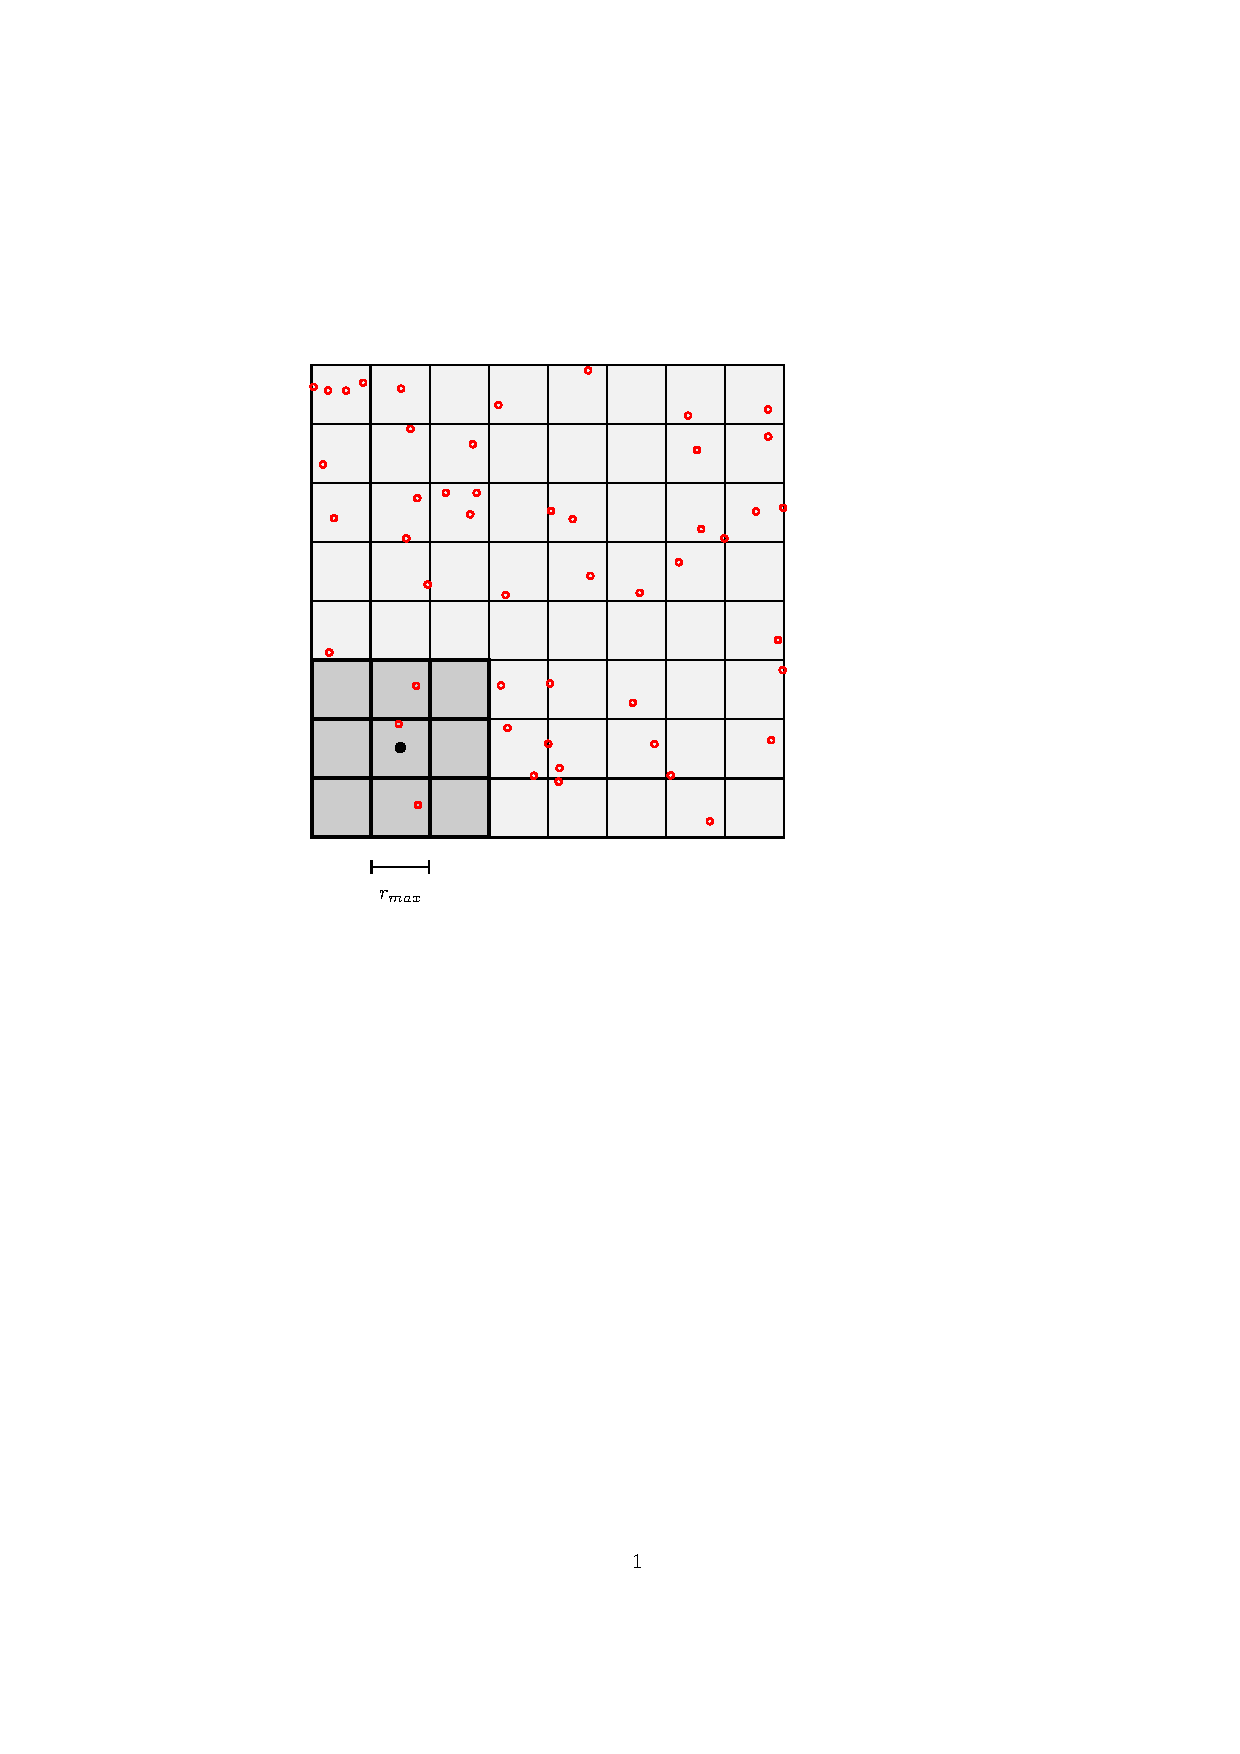
\includegraphics[width=\textwidth,clip=true]{tikz_grid}
\caption{A 2-D grid showing the bin-lattice partitioning scheme. The bigger square show the entire
domain, the red circles show a random distribution of 100 particles. Let's say we want to compute all pairs
for the target blue point, then we would only have to consider red points that are within one cell (the dark shaded region).
A circle with radius \rmax is also drawn to shown the actual pairs that will eventually count in the correlation function.}
\label{fig:grid}
\end{figure}


\subsection{How to Maintain Cache Locality within the Grid}
For all pairs around a given target galaxy, we need to compute distances to all points within all neighbouring 3-d cells.
We ensure that the particle locations are contiguous by moving them into the following \texttt{C struct} in the order in which they arrive.
\begin{lstlisting}[label={code:celldefn},caption={Definition of the cellarray structure. This 
structure contains the \texttt{X/Y/Z} positions of all the particles that are in one 3-D cell. }]
typedef struct{
  DOUBLE *x;
  DOUBLE *y;
  DOUBLE *z;
  int64_t nelements;
} cellarray;
\end{lstlisting}
The code \texttt{gridlink.c} takes in an input list of 3 arrays \texttt{X/Y/Z} and grids them into a regular 3-D grid using the specified bins parameter
\texttt{max\_x\_size} or \texttt{max\_y\_size} or \texttt{max\_z\_size} for the \texttt{X/Y/Z} axes respectively. \footnote{In practice, the bins may be further 
subdivided using the corresponding bin refine factors. These bin refine factors seem to influence runtime the most, you should experiment with a few values of 
\texttt{bin\_refine\_factor} and \texttt{zbin\_refine\_factor} to see what produces the best runtimes for your typical scenario.}
Once the number of grid cells along each axes has been determined, we allocate memory for the \texttt{struct lattice}. This \texttt{struct lattice} is a 
declared as an 1-D array; the conversion from the three indices in 3-D (\texttt{ix,iy,iz}) to a single index (\texttt{index}) happens through the last 
line in Listing~\ref{code:onedim_index}. Such an 1-D array for \texttt{struct lattice} gives much better OpenMP scaling.   
\begin{lstlisting}[label={code:onedim_index},caption={Accessing as \texttt{lattice[index]} rather than \texttt{lattice[ix][iy][iz]}.}]
int64_t totncells  = nmesh_x * nmesh_y * nmesh_z;
cellarray *lattice  = my_malloc(sizeof(cellarray), totncells);
int64_t *nallocated = my_malloc(sizeof(*nallocated), totncells);
int64_t index = ix*nmesh_y*nmesh_z + iy*nmesh_z + iz;
\end{lstlisting}
Now that we know the total number of cells in the entire domain, we need to allocated memory to store the particles in each cell. However, there is no way to 
know the exact number of particles in each cell without processing the entire data-set; so, we pre-allocate with an estimate of the expected number of particles from the 
volume of each 3-D cell (assuming a random distribution). Then, we can allocate memory for each of the \texttt{X/Y/Z} arrays inside each 3-D cell:
\begin{lstlisting}[label={code:malloc_cellarray},caption={Pre-allocating memory for the \texttt{X/Y/Z} arrays in \texttt{struct cellarray}.}]
for (int64_t index=0;index<totncells;index++) {
  lattice[index].x = my_malloc(sizeof(DOUBLE),expected_n);
  lattice[index].y = my_malloc(sizeof(DOUBLE),expected_n);
  lattice[index].z = my_malloc(sizeof(DOUBLE),expected_n);
  lattice[index].nelements=0;
  nallocated[index] = expected_n;
}
\end{lstlisting}
Here, \texttt{nallocated} is an array that keeps track of the amount of memory alread allocated for each cell. After this step, all cells have been allocated memory for \texttt{expected\_n} 
particles. Now, we can begin to process the individual particles and assigning them to the 3-D cells (if enough memory has already been allocated to assign the new particle). 
\begin{lstlisting}[label={code:assign_to_cellarray},caption={Assigning the particles to the \texttt{struct cellarray} in the cell.}]
for (int64_t i=0;i<np;i++)  {
  ix=(int)((x[i]-xmin)*xinv) ;
  iy=(int)((y[i]-ymin)*yinv) ;
  iz=(int)((z[i]-zmin)*zinv) ;

  int64_t index = ix*nmesh_y*nmesh_z + iy*nmesh_z + iz;
  
  if(lattice[index].nelements == nallocated[index]) {
    expected_n = nallocated[index]*MEMORY_INCREASE_FAC;
    
    lattice[index].x = my_realloc(lattice[index].x ,sizeof(DOUBLE),expected_n,''lattice.x'');
    lattice[index].y = my_realloc(lattice[index].y ,sizeof(DOUBLE),expected_n,''lattice.y'');
    lattice[index].z = my_realloc(lattice[index].z ,sizeof(DOUBLE),expected_n,''lattice.z'');
    
    nallocated[index] = expected_n;
  }
  int64_t ipos=lattice[index].nelements;
  lattice[index].x[ipos] = x[i];
  lattice[index].y[ipos] = y[i];
  lattice[index].z[ipos] = z[i];
  lattice[index].nelements++;
}
\end{lstlisting}
The loop goes over all of the particles and calculates the corresponding 3-D cell indices --- \texttt{ix,iy,iz}. With these 3 variables, the corresponding 1-D index, \texttt{index}, can be 
calculated. The next lines check (and reallocate memory, if necessary) to ensure that enough memory has been allocated to the \texttt{struct lattice[index]} to accommodate this new particle. 
The last 5 lines are simply assigning the particle into the appropriate \texttt{struct lattice[index]}. Once all the particles have been assigned, the cells contain contiguous \texttt{X/Y/Z} 
arrays describing the original particle distribution. 

\subsection{The Pair-Counting Algorithms}
After running through \texttt{gridlink}, the particle distribution is stored in contiguous \texttt{X/Y/Z} inside the 1-D array of \texttt{struct cellarray}. To find all 
possible pairs, we first need to loop over all particles in the first data-set. 
\begin{lstlisting}[label={code:loop_over_first_cells},caption={Looping over all cells in the first data-set.}]
for (int64_t index1=0;index1<totncells;index1++) {
  const cellarray *first = &lattice1[index1];
  const DOUBLE *x1 = first->x;
  const DOUBLE *y1 = first->y;
  const DOUBLE *z1 = first->z;
}
\end{lstlisting}
Now, we have the target cell pointer and the associated \texttt{x1/y1/z1} array pointers. Next, we need to get the indices for the neighbouring cells in 3-D. In order to do that, first 
the 1-D index, \texttt{index1} needs to be converted into a set of three 3-D indices, \texttt{ix, iy, iz}. Listing~\ref{code:finding_3D_index_first} shows the conversion from 
the 1-D index to the corresponding 3-D indices. 
\begin{lstlisting}[label={code:finding_3D_index_first},caption={Reconstructing 3-D index for \texttt{first} cell in the first data-set.}]
const int iz = index1 % nmesh_z ;
const int ix = index1 / (nmesh_z * nmesh_y) ;
const int iy = (index1 - iz - ix*nmesh_z*nmesh_y)/nmesh_z ;
\end{lstlisting}
After executing the code segment in Listing~\ref{code:finding_3D_index_first}, we have the full 3-D indices for the target cell. Now, we have to find all of the indices 
for the neighbouring cells that can potentially satisfy the \rmax constraint. This requires considering all 3-D cells that are located within \texttt{bin\_refine\_factor} of 
the target cell (for each dimension). Since the target cell, \texttt{first} has a 3-D X index of \texttt{ix}, this means all cells that have X indices in the range 
\texttt{ix $\pm$ bin\_refine\_factor} can potentially have pairs that satisfy the \rmax constraint. However, in case of PERIODIC boundary conditions, we also have 
to ensure that the indices (and the actual particle positions) wrap around on the other side of the cube. Listing~\ref{code:looping_over_neighbouring_cells} shows 
how the looping over neighbouring cells is done for the X dimension. Similar segments follow in the actual code for the Y/Z dimensions. 
\begin{lstlisting}[label={code:looping_over_neighbouring_cells},caption={Looping over all the neighbouring cells and taking care of PERIODIC boundary conditions.}]
for(int iix=-bin_refine_factor;iix<=bin_refine_factor;iix++){
  int iiix;
#ifdef PERIODIC
  DOUBLE off_xwrap=0.0;
  if(ix + iix >= nmesh_x) {
    off_xwrap = -xdiff;
  } else if (ix + iix < 0) {
    off_xwrap = xdiff;
  }
  iiix=(ix+iix+nmesh_x)%nmesh_x;
#else
  iiix = iix+ix;
  if(iiix < 0 || iiix >= nmesh_x) {
    continue;
  }
#endif
  (*@{\Large$\vdots$}@*)
  (*@{\normalsize \texttt{Similar chunks of code for Y/Z.}}@*)
  (*@{\Large$\vdots$}@*)
  const int64_t index2 = iiix*nmesh_y*nmesh_z + iiiy*nmesh_z + iiiz;
\end{lstlisting}
Once all of the three 3-D indices for the neighbouring cell has been determined, we can reconstruct the 1-D index, \texttt{index2} for that cell. With this 1-D index, we can 
create a pointer, \texttt{second}, that contains the \texttt{cellarray pointer} to the neighbouring cell. In Listing~\ref{code:dereference_second_cell}, we show 
how the neighbouring cell and the associated \texttt{x2/y2/z2} array pointers are defined. 
\begin{lstlisting}[label={code:dereference_second_cell},caption={Dereferencing the pointers for the neighbouring (\texttt{second}) cell under consideration.}]
const cellarray *second = &lattice2[index2];
const DOUBLE *x2 = second->x;
const DOUBLE *y2 = second->y;
const DOUBLE *z2 = second->z;
\end{lstlisting}
At this point, we have a set of \texttt{x1/y/1/z1} arrays with \texttt{first->nelements} elements representing the first data-set. We also have another set of \texttt{x2/y2/z2} arrays with \texttt{second->nelements} 
elements representing the second data-set. Now, we have to compute all possible pair-wise separations between these two data-sets. We begin with a loop over the elements in 
\texttt{first}:
\begin{lstlisting}[label={code:looping_over_first_particles},caption={Looping over all particles in the \texttt{first} cell and accounting for PERIODIC boundary conditions.}]
for(int64_t i=0;i<first->nelements;i++) {
  DOUBLE x1pos=x1[i];
  DOUBLE y1pos=y1[i];
  DOUBLE z1pos=z1[i];
#ifdef PERIODIC
  x1pos += off_xwrap;
  y1pos += off_ywrap;
  z1pos += off_zwrap;
#endif
\end{lstlisting}
If PERIODIC boundary conditions are enabled, then \texttt{off\_xwrap}, \texttt{off\_ywrap} and \texttt{off\_zwrap} have been declared and initialized in Listing~\ref{code:looping_over_neighbouring_cells}.
By wrapping the elements if the first data-set, we can avoid the wrapping operations in the \texttt{j-loop} over all particles in \texttt{second}. 
\begin{lstlisting}[label={code:looping_over_second_particles},caption={AVX intrinsics for looping over all particles in the \texttt{second} cell. PERIODIC boundary conditions have 
already been accounted for in \texttt{x1pos,y1pos,z1pos} variables.}]
const AVX_FLOATS m_x1pos = AVX_SET_FLOAT(x1pos);
const AVX_FLOATS m_y1pos = AVX_SET_FLOAT(y1pos);
const AVX_FLOATS m_z1pos = AVX_SET_FLOAT(z1pos);

int64_t j;
for(j=0;j<=(second->nelements-NVEC);j+=NVEC) {
  const AVX_FLOATS x2pos = AVX_LOAD_FLOATS_UNALIGNED(&x2[j]);
  const AVX_FLOATS y2pos = AVX_LOAD_FLOATS_UNALIGNED(&y2[j]);
  const AVX_FLOATS z2pos = AVX_LOAD_FLOATS_UNALIGNED(&z2[j]);
  
  const AVX_FLOATS m_xdiff = AVX_SUBTRACT_FLOATS(m_x1pos,x2pos);
  const AVX_FLOATS m_ydiff = AVX_SUBTRACT_FLOATS(m_y1pos,y2pos);
  const AVX_FLOATS m_zdiff = AVX_SUBTRACT_FLOATS(m_z1pos,z2pos);
\end{lstlisting}  

The three codes \xir, \xirppi and \wprp diverge somewhat after this point. For \xir, we need to calculate the full 3-D separation, whereas for \xirppi and \wprp 
the separation is the projected distance. I will discuss further implementations in the following sub-sections dedicated to each code. 
\subsubsection{Pair-counting for \texorpdfstring{\xir}{xi(r)}}\label{section:pair_counting_r}
Pair-counting for \xir is the most straight-forward. The squared 3-D separation, \texttt{r2}, is simply the sum of the squared differences in 
each \texttt{X/Y/Z} dimensions. 
\begin{lstlisting}[label={code:r2_xi},caption={Calculating squared separations in \xir.}]
const AVX_FLOATS m_xdiff_sqr = AVX_SQUARE_FLOAT(m_xdiff);
const AVX_FLOATS m_ydiff_sqr = AVX_SQUARE_FLOAT(m_ydiff);
const AVX_FLOATS m_zdiff_sqr = AVX_SQUARE_FLOAT(m_zdiff);
const AVX_FLOATS m_xydiff_sqr_sum = AVX_ADD_FLOATS(m_xdiff_sqr,m_ydiff_sqr);
AVX_FLOATS r2 = AVX_ADD_FLOATS(m_zdiff_sqr,m_xydiff_sqr_sum);
\end{lstlisting}
Once all the \texttt{NVEC} separations have been computed, we use bit-masks to check if any separations fall 
within the range \texttt{sqr\_rpmin} and \texttt{sqr\_rpmax}. If not, we \texttt{continue} with the \texttt{j-loop}. 
\begin{lstlisting}[label={code:masks_xi},caption={Bit-masks in \xir.}]
m_mask_left = AVX_COMPARE_FLOATS(r2,m_sqr_rpmax,_CMP_LT_OS);
if(AVX_TEST_COMPARISON(m_mask_left) == 0) {
  continue;
}

const AVX_FLOATS m_mask = AVX_BITWISE_AND(m_mask_left, AVX_COMPARE_FLOATS(r2, m_sqr_rpmin, _CMP_GE_OS));
if(AVX_TEST_COMPARISON(m_mask) == 0) {
  continue;
}
r2 = AVX_BLEND_FLOATS_WITH_MASK(m_sqr_rpmax, r2, m_mask);
m_mask_left = AVX_COMPARE_FLOATS(r2,m_sqr_rpmax,_CMP_LT_OS);
\end{lstlisting}
If the code reaches past this bit-mask section, then at least one separation is within range. In that case, we use the 
code in Listing~\ref{code:updating_histogram} to update the \texttt{npairs} array (and the \texttt{rpavg} array if 
OUTPUT\_RPAVG is enabled). 

\subsubsection{Pair-separations for the projected correlation functions \texorpdfstring{\xirppi,\wprp}{xi(rp,pi), wp(rp)}}
Listing~\ref{code:r2_projected} shows the squared distance calculation for \xirppi and \wprp. \texttt{r2} is simply 
the projected separation in the \texttt{X-Y} plane.
\begin{lstlisting}[label={code:r2_projected},caption={Calculating squared separations in \xirppi and \wprp.}]
const AVX_FLOATS m_xdiff_sqr = AVX_SQUARE_FLOAT(m_xdiff);
const AVX_FLOATS m_ydiff_sqr = AVX_SQUARE_FLOAT(m_ydiff);
AVX_FLOATS r2 = AVX_ADD_FLOATS(m_xdiff_sqr,m_ydiff_sqr);
\end{lstlisting}

\subsubsection{Pair-counting for \texorpdfstring{\xirppi}{xi(rp,pi)}}\label{section:pair_counting_rp_pi}
\begin{lstlisting}[label={code:masks_xirppi},caption={Bit-masks in \xirppi.}]
const AVX_FLOATS m_mask_pimax = AVX_COMPARE_FLOATS(m_zdiff,m_pimax,_CMP_LT_OS);
const int test = AVX_TEST_COMPARISON(m_mask_pimax);
if(test == 0) {
  continue;
}

const AVX_FLOATS m1 = AVX_COMPARE_FLOATS(r2,m_sqr_rpmin,_CMP_GE_OS);
r2 = AVX_BLEND_FLOATS_WITH_MASK(m_sqr_rpmax,r2,m_mask_pimax);

m_mask_left = AVX_COMPARE_FLOATS(r2,m_sqr_rpmax,_CMP_LT_OS);
const AVX_FLOATS m_mask = AVX_BITWISE_AND(m1,m_mask_left);
int test1 = AVX_TEST_COMPARISON(m_mask);
if(test1 == 0) {
  continue;
}
m_zdiff = AVX_BLEND_FLOATS_WITH_MASK(m_pimax, m_zdiff, m_mask);
#ifdef OUTPUT_RPAVG
union_mDperp.m_Dperp = AVX_SQRT_FLOAT(r2);
#endif
union_pibin.m_ibin = AVX_TRUNCATE_FLOAT_TO_INT(AVX_MULTIPLY_FLOATS(m_zdiff,m_inv_dpi));
\end{lstlisting}
In the \xirppi code, we have to update a two dimensional \texttt{npairs($r_p$,$\pi$)} array. This means we can not directly update 
the \texttt{npairs} matrix and instead have to use a separate loop (this loop is typically only invoked for \xir and \wprp 
when OUTPUT\_RPAVG is enabled). As a result of this extra loop, \xirppi is $2-3\times$ slower than \xir and \wprp. 

\begin{lstlisting}[label={code:updating_histogram_xirppi},caption={Updating the \texttt{npairs} matrix in \xirppi.}]
for(int jj=0;jj<NVEC;jj++) {
  int rpbin = union_rpbin.ibin[jj];
  int pibin = union_pibin.ibin[jj];
  int ibin = rpbin*(npibin+1) + pibin;
  npairs[ibin]++;
#ifdef OUTPUT_RPAVG
  rpavg [ibin] += union_mDperp.Dperp[jj];
#endif
}
\end{lstlisting}

\subsubsection{Pair-counting for \texorpdfstring{\wprp}{wp(rp)}}\label{section:pair_counting_wp}
Since the pair-counting in \wprp always assumes PERIODIC boundary conditions {\em and} only computes an auto-correlation, extra optimizations are possible in the
\wprp calculation. First, each individual cell in the \texttt{struct lattice} elements are sorted based on their \texttt{Z} arrays. The \texttt{X/Y} arrays are 
also re-ordered simultaneously. Once all the \texttt{Z} values inside a cell have been sorted, we can avoid double-counting the pairs by changing the \texttt{iiz loop}
to be:
\begin{lstlisting}[label={code:loop_optimization_wp},caption={Optimizing the loop over neighbouring cells \texttt{z} in \wprp.}]
for(int iiz=0;iiz<=zbin_refine_factor;iiz++)

(*@{\Large instead of }@*)

for(int iiz=-zbin_refine_factor;iiz<=zbin_refine_factor;iiz++)
\end{lstlisting}
Another advantage of sorting the \texttt{Z} values is earlier termination inside the actual calculation. The Listing~\ref{code:calculating_separations_wp} shows 
how to break early from the \texttt{j-loop}. Since the \texttt{z2} values are always stored in increasing order, if {\em all} values of \texttt{zdiff:=z2[j:j+NVEC-1]-z1}
are greater than \pimax, then none of the \texttt{zdiff} values in future iterations of the \texttt{j-loop} can be smaller than \pimax. When the code encounters 
such a scenario, it updates the \texttt{j} variable to \texttt{second->nelements} to ensure that the serial section of the code is not executed and breaks out the 
AVX \texttt{j-loop}. 
\begin{lstlisting}[label={code:calculating_separations_wp},caption={AVX intrinsics for calculating separations in \wprp and checking for early termination.}]
const AVX_FLOATS m_zdiff = AVX_SUBTRACT_FLOATS(m_z2,m_zpos);//z2[j:j+NVEC-1] - z1                                                                                                                                        
AVX_FLOATS m_mask_pimax = AVX_COMPARE_FLOATS(m_zdiff,m_pimax,_CMP_LT_OS);
const int test = AVX_TEST_COMPARISON(m_mask_pimax);
if(test == 0) {
  j = second->nelements;
  break;
}
\end{lstlisting}

\subsection{AVX intrinsics to update the \texttt{npairs} histogram}
This section explains the AVX intrinsics used to update the pair-counts histogram, \texttt{npairs}.\footnote{The thread-local version in \wprp is called \texttt{local\_npair}.}
If the code execution reaches this loop, at least one (squared) pair separation falls within the range \texttt{sqr\_rpmin} and \texttt{sqr\_rpmax}, where \texttt{sqr\_rpmin} 
is the squared lower radial limit of the first bin and \texttt{sqr\_rpmax} is the squared upper limit of the last bin (equivalent to \rmax$^2$ in this user-guide). 
Since the pairs are more likely to occur in the largest separation bins, the loop goes backwards from the last bin to the first and uses early loop-termination in case
all possible pairs have already been accounted for. 
\begin{lstlisting}[label={code:updating_histogram},caption={AVX intrinsics for updating the \texttt{npairs} histgram for \xir and \wprp.}]
for(int kbin=nrpbin-1;kbin>=1;kbin--) {
  const AVX_FLOATS m1 = AVX_COMPARE_FLOATS(r2,m_rupp_sqr[kbin-1],_CMP_GE_OS);
  const AVX_FLOATS m_bin_mask = AVX_BITWISE_AND(m1,m_mask_left);
  m_mask_left = AVX_COMPARE_FLOATS(r2,m_rupp_sqr[kbin-1],_CMP_LT_OS);
  const int test2  = AVX_TEST_COMPARISON(m_bin_mask);
  npairs[kbin] += AVX_BIT_COUNT_INT(test2);
#ifdef OUTPUT_RPAVG
  m_rpbin = AVX_BLEND_FLOATS_WITH_MASK(m_rpbin,m_kbin[kbin], m_bin_mask);
#endif
  const int test3 = AVX_TEST_COMPARISON(m_mask_left);
  if(test3 == 0) break;
}
\end{lstlisting}
Note that \texttt{rupp\_sqr} (and its AVX equivalent, \texttt{m\_rupp\_sqr}) contains the squared upper limits for the bins. Thus, when considering bin \texttt{kbin}, 
\texttt{m\_rupp\_sqr[kbin-1]} gives the squared lower radial limit for the bin while \texttt{m\_rupp\_sqr[kbin]} gives the squared upper limit for bin \texttt{kbin}. 
Here, \texttt{m1} is the mask that contains all separations that satisfy \texttt{r2 $\geq$ rupp\_sqr[kbin-1]}, while the mask \texttt{m\_mask\_left} contains 
those squared separations that satisfy \texttt{r2 < rupp\_sqr[kbin]}. Note, that \texttt{m\_mask\_left} is either computed before entering the \texttt{kbin} 
loop or during a previous iteration of the same \texttt{kbin} loop. The AVX variable \texttt{m\_bin\_mask} then contains the bitwise and of \texttt{m1} and 
\texttt{m\_mask\_left} -- the mask for the squared separations that fall into \texttt{kbin}. The variable \texttt{test2} contains an integer composed of 
the upper set-bits of the mask \texttt{m\_bin\_mask} -- thus, contains only 4/8 useful bits for \texttt{float/double} precision calculations respectively. The 
\texttt{npairs} pair-counts is then updated using a hardware \texttt{popcnt} instruction. The last two lines check if there are any more pairs left that satisfy 
the lower bin-ranges; if not, the loop is terminated with a \texttt{break} statement. 


\section{Calling the C Libraries}
All of the correlation function codes create a corresponding \texttt{static} library rather than a \texttt{dynamic/shared} library. This was a design decision intended 
to minimize path-issues for the end-user. After the libraries have been created, it is fairly straightforward to use them in an external \texttt{C/python} code.  
Be absolutely sure to pass arrays for the correct type -- float arrays if you did not use DOUBLE\_PREC (default) or double arrays if you did use DOUBLE\_PREC. 
Also, only include headers from the \texttt{xi\_theory/include} directory -- those headers correspond to the actual static library. {\em DO NOT include} 
the header files from the \texttt{xi\_of\_r}/\texttt{xi\_rp\_pi}/\texttt{wp} directories -- these headers do not contain the correct function signature for 
the compilation flags used to generate the static libraries. 

\subsection{C bindings}
The \texttt{examples} contains the files \texttt{run\_correlations.c} that shows how to use the three types of correlation function libraries from C. Essentially, the process 
consists of including the appropriate header file and passing the arrays ({\em of the correct \texttt{float/double} type}) into the functions. Make sure to include the static 
library in the linking step to create a stand-alone executable (see the \texttt{Makefile} in the \texttt{examples} directory). 

\subsubsection{API for \texorpdfstring{\xir}{xi(r)}}
The interface for the 3-D correlation function, \xir, is through the \texttt{countpairs} function. Here is 
the corresponding function signature:
\begin{lstlisting}[label={code:API_DD},caption={API for the 3-D \xir.}]
results_countpairs * countpairs(
const int64_t ND1, const DOUBLE * const X1, const DOUBLE * const Y1, const DOUBLE  * const Z1,
const int64_t ND2, const DOUBLE * const X2, const DOUBLE * const Y2, const DOUBLE  * const Z2,
#ifdef USE_OMP
const int numthreads,
#endif
const int autocorr,
const char *binfile);
\end{lstlisting}

The parameters to the function are:
\begin{itemize}
\item \texttt{ND1} -- number of elements in the first data-set.
\item \texttt{X1}  -- the array of X-values in the first data-set.
\item \texttt{Y1}  -- the array of Y-values in the first data-set.
\item \texttt{Z1}  -- the array of Z-values in the first data-set.
\item \texttt{ND2} -- number of elements in the second data-set.
\item \texttt{X2}  -- the array of X-values in the second data set.
\item \texttt{Y2}  -- the array of Y-values in the second data set.
\item \texttt{Z2}  -- the array of Z-values in the second data set.
\item \texttt{numthreads} -- the number of threads to use (if USE\_OMP is enabled in \texttt{common.mk}).
\item \texttt{autocorr} -- if an auto-correlation is being calculated (1 implies auto-correlation, flag is used for some runtime optimizations).
\item \texttt{binfile} -- file name that contains the radial bins. See Section~\ref{section:bins} for details on how to create this file.
\end{itemize}

The output from \texttt{countpairs} is contained in \texttt{struct results\_countpairs}. The structure
definition is:
\begin{lstlisting}[label={code:API_DD_struct},caption={Structure definition for the output of \xir.}]
typedef struct{
  uint64_t *npairs;
  DOUBLE *rupp;
  DOUBLE *rpavg;
  int nbin;
} results_countpairs;

void free_results(results_countpairs **results);
\end{lstlisting}

The fields in the structure correspond to:
\begin{itemize}
\item \texttt{npairs} -- array containing the pair-counts. 
\item \texttt{rupp}   -- array containing the upper limits of the bins. \texttt{rupp[0]} gives the lower-limit of the first radial bin. 
\item \texttt{rpavg}  -- array containing the average value of the separations for all the pairs that fell into the bin. Will contain 
meaningful values if OUTPUT\_RPAVG is defined in \texttt{common.mk}; identically \texttt{0.0} otherwise. 
\item \texttt{nbin}   -- the number of radial bins used. Note that the actual pair-counts are stored in the index range \texttt{[1,nbin-1]}. The
zero'th bin contains garbage for all of the arrays in this \texttt{struct results\_countpairs}.
\end{itemize}
After the results structure has been used, use \texttt{free\_results(\&results\_countpairs)} to free allocated memory. 

\subsubsection{API for \texorpdfstring{\xirppi}{xi(rp,pi)}}
The interface for the 2-D correlation function, \xirppi, is through the \texttt{countpairs\_rp\_pi} function. Here is 
the corresponding function signature:
\begin{lstlisting}[label={code:API_DDrppi},caption={API for the 2-D \xirppi}]
results_countpairs_rp_pi * countpairs_rp_pi(
const int64_t ND1, const DOUBLE *X1, const DOUBLE *Y1, const DOUBLE *Z1,
const int64_t ND2, const DOUBLE *X2, const DOUBLE *Y2, const DOUBLE *Z2,
#ifdef USE_OMP
const int numthreads,
#endif
const int autocorr,
const char *binfile,
const double pimax);
\end{lstlisting}

The parameters to the function are:
\begin{itemize}
\item \texttt{ND1} -- number of elements in the first data-set.
\item \texttt{X1}  -- the array of X-values in the first data-set.
\item \texttt{Y1}  -- the array of Y-values in the first data-set.
\item \texttt{Z1}  -- the array of Z-values in the first data-set.
\item \texttt{ND2} -- number of elements in the second data-set.
\item \texttt{X2}  -- the array of X-values in the second data set.
\item \texttt{Y2}  -- the array of Y-values in the second data set.
\item \texttt{Z2}  -- the array of Z-values in the second data set.
\item \texttt{numthreads} -- the number of threads to use (if USE\_OMP is enabled in \texttt{common.mk}).
\item \texttt{autocorr} -- if an auto-correlation is being calculated (1 implies auto-correlation, flag is used for some runtime optimizations).
\item \texttt{binfile} -- file name that contains the radial bins. See Section~\ref{section:bins} for details on how to create this file.
\item \texttt{pimax} -- the maximum line-of-sight distance (assumed to be the \texttt{Z} axis) to use. 
\end{itemize}

The output from \texttt{countpairs\_rp\_pi} is contained in \texttt{struct results\_countpairs\_rp\_pi}. The structure
definition is:
\begin{lstlisting}[label={code:API_DDrppi_struct},caption={Structure definition for the output of \xirppi}]
typedef struct{
  uint64_t *npairs;
  DOUBLE *rupp;
  DOUBLE *rpavg;
  DOUBLE pimax;
  int nbin;
  int npibin;
} results_countpairs_rp_pi;

void free_results_rp_pi(results_countpairs_rp_pi **results);
\end{lstlisting}

The fields in the structure correspond to:
\begin{itemize}
\item \texttt{npairs} -- array containing the pair-counts.  Number of elements in the array is \texttt{(npibin+1)$\times$(nbin+1)}.
\item \texttt{rupp}   -- array containing the upper limits of the bins. \texttt{rupp[0]} gives the lower-limit of the first radial bin. Number of elements 
in the array is \texttt{nbin}. 
\item \texttt{rpavg}  -- array containing the average value of the separations for all the pairs that fell into the bin. Will contain 
meaningful values if OUTPUT\_RPAVG is defined in \texttt{common.mk}; identically \texttt{0.0} otherwise. Number of elements in the array is \texttt{(npibin+1)$\times$(nbin+1)}.
\item \texttt{pimax}  -- the maximum line-of-sight distance used in the bins. 
\item \texttt{nbin}   -- the number of radial bins used. Note that the actual pair-counts are stored in the index range \texttt{[1,nbin-1]}. The
zero'th bin contains garbage for all of the arrays in this \texttt{struct results\_countpairs\_rp\_pi}.
\item \texttt{npibin} -- the number of $\pi$ bins used. The total number of elements in the arrays in the \texttt{struct countpair\_rp\_pi} is 
\texttt{(npibin+1)$\times$(nbin+1)}. As usual, meaningful data is only contained in the radial bin range \texttt{[1,nbin-1]}. 
\end{itemize}
After the results structure has been used, use \texttt{free\_results\_rp\_pi(\&results\_countpairs\_rp\_pi)} to free allocated memory. 

\subsubsection{API for \texorpdfstring{\wprp}{wp(rp)}}
The interface for the projected correlation function, \wprp, is through the \texttt{countpairs\_wp} function. The code 
{\em always} uses PERIODIC boundary conditions, irrespective of the settings in \texttt{common.mk}. Here is 
the corresponding function signature\footnote{The \texttt{X1/Y1/Z1} arrays are not 
declared with \texttt{const} qualifiers because I sort those arrays on \texttt{Z} in the 
\texttt{countpairs\_wp} function.}:
\begin{lstlisting}[label={code:API_wp},caption={API for the \wprp.}]
results_countpairs_wp *countpairs_wp(
const int64_t ND1, DOUBLE * restrict X1, DOUBLE * restrict Y1, DOUBLE * restrict Z1,
const double boxsize, 
#ifdef USE_OMP
const int numthreads,
#endif
const char *binfile,
const double pimax);
\end{lstlisting}

The parameters to the function are:
\begin{itemize}
\item \texttt{ND1} -- number of elements in the data-set.
\item \texttt{X1}  -- the array of X-values in the data-set.
\item \texttt{Y1}  -- the array of Y-values in the data-set.
\item \texttt{Z1}  -- the array of Z-values in the data-set.
\item \texttt{boxsize}  -- the boxsize that fully contains the \texttt{X/Y/Z} values. 
\item \texttt{numthreads} -- the number of threads to use (if USE\_OMP is enabled in \texttt{common.mk}).
\item \texttt{binfile} -- file name that contains the radial bins. See Section~\ref{section:bins} for details on how to create this file.
\item \texttt{pimax} -- the maximum line-of-sight distance (assumed to be the \texttt{Z} axis) to use. 
\end{itemize}

The output from \texttt{countpairs\_wp} is contained in \texttt{struct results\_countpairs\_wp}. The structure definition is:
\begin{lstlisting}[label={code:API_wp_struct},caption={Structure definition for the output of \wprp}]
typedef struct{
  uint64_t *npairs;
  DOUBLE *wp;
  DOUBLE *rupp;
  DOUBLE *rpavg;
  DOUBLE pimax;
  int nbin;
} results_countpairs_wp;

void free_results_wp(results_countpairs_wp **results);
\end{lstlisting}

The fields in the structure correspond to:
\begin{itemize}
\item \texttt{npairs} -- array containing the pair-counts.  Number of elements in the array is \texttt{nbin}.
\item \texttt{wp}     -- array containing the actual \texttt{wp} values. 
\item \texttt{rupp}   -- array containing the upper limits of the bins. \texttt{rupp[0]} gives the lower-limit of the first radial bin. Number of elements 
in the array is \texttt{nbin}. 
\item \texttt{rpavg}  -- array containing the average value of the separations for all the pairs that fell into the bin. Will contain 
meaningful values if OUTPUT\_RPAVG is defined in \texttt{common.mk}; identically \texttt{0.0} otherwise. Number of elements in the array is \texttt{nbin}.
\item \texttt{pimax}  -- the maximum line-of-sight distance used in the bins. 
\item \texttt{nbin}   -- the number of radial bins used. Note that the actual pair-counts are stored in the index range \texttt{[1,nbin-1]}. The
zero'th bin contains garbage for all of the arrays in this \texttt{struct results\_countpairs\_wp}.
\end{itemize}
After the results structure has been used, use \texttt{free\_results\_wp(\&results\_countpairs\_wp)} to free allocated memory. 

\subsection{Python Bindings}
The \texttt{python\_bindings} directory contains python bindings for python 2.x. Note that python3 is not supported out of the box\footnote{In the future, I might switch to 
cython to cover both python2 and python3}. If all went well, then typing \texttt{python call\_correlation\_functions.py} should run the example python code. If you get 
an error (and you are on a MAC), then refer to Section~\ref{section:mac} or the FAQ. 
If you edit the \texttt{common.mk} file and compile for \texttt{double precision} arithmetic, then be sure to change the line \texttt{dtype=np.float32} to 
\texttt{dtype=np.float64}. Otherwise, you will get a \texttt{TypeError} at runtime. 

\stdsection{Benchmarks \& Scaling}
In this section we present the runtimes and scalings for different number of particles, \rmax and OpenMP threads for the codes. 
For all of the scaling tests, only an auto-correlation calculation was used and the fiducial catalog contains $\sim 1.2$ million 
galaxies on a periodic cube of side 420 \hMpc. 

\subsection{Scaling with Number of Particles}
In Fig.~\ref{fig:scaling_numpart}, we show the scaling for the three codes with the number of particles. For this scaling, we subsampled 
the fiducial mock to attain 10 logarithmic steps in particle number ranging from $1.2\times10^4$ to $1.2\times10^6$. All the timings are 
generateed using 1 thread. 
\begin{figure}[htbp]
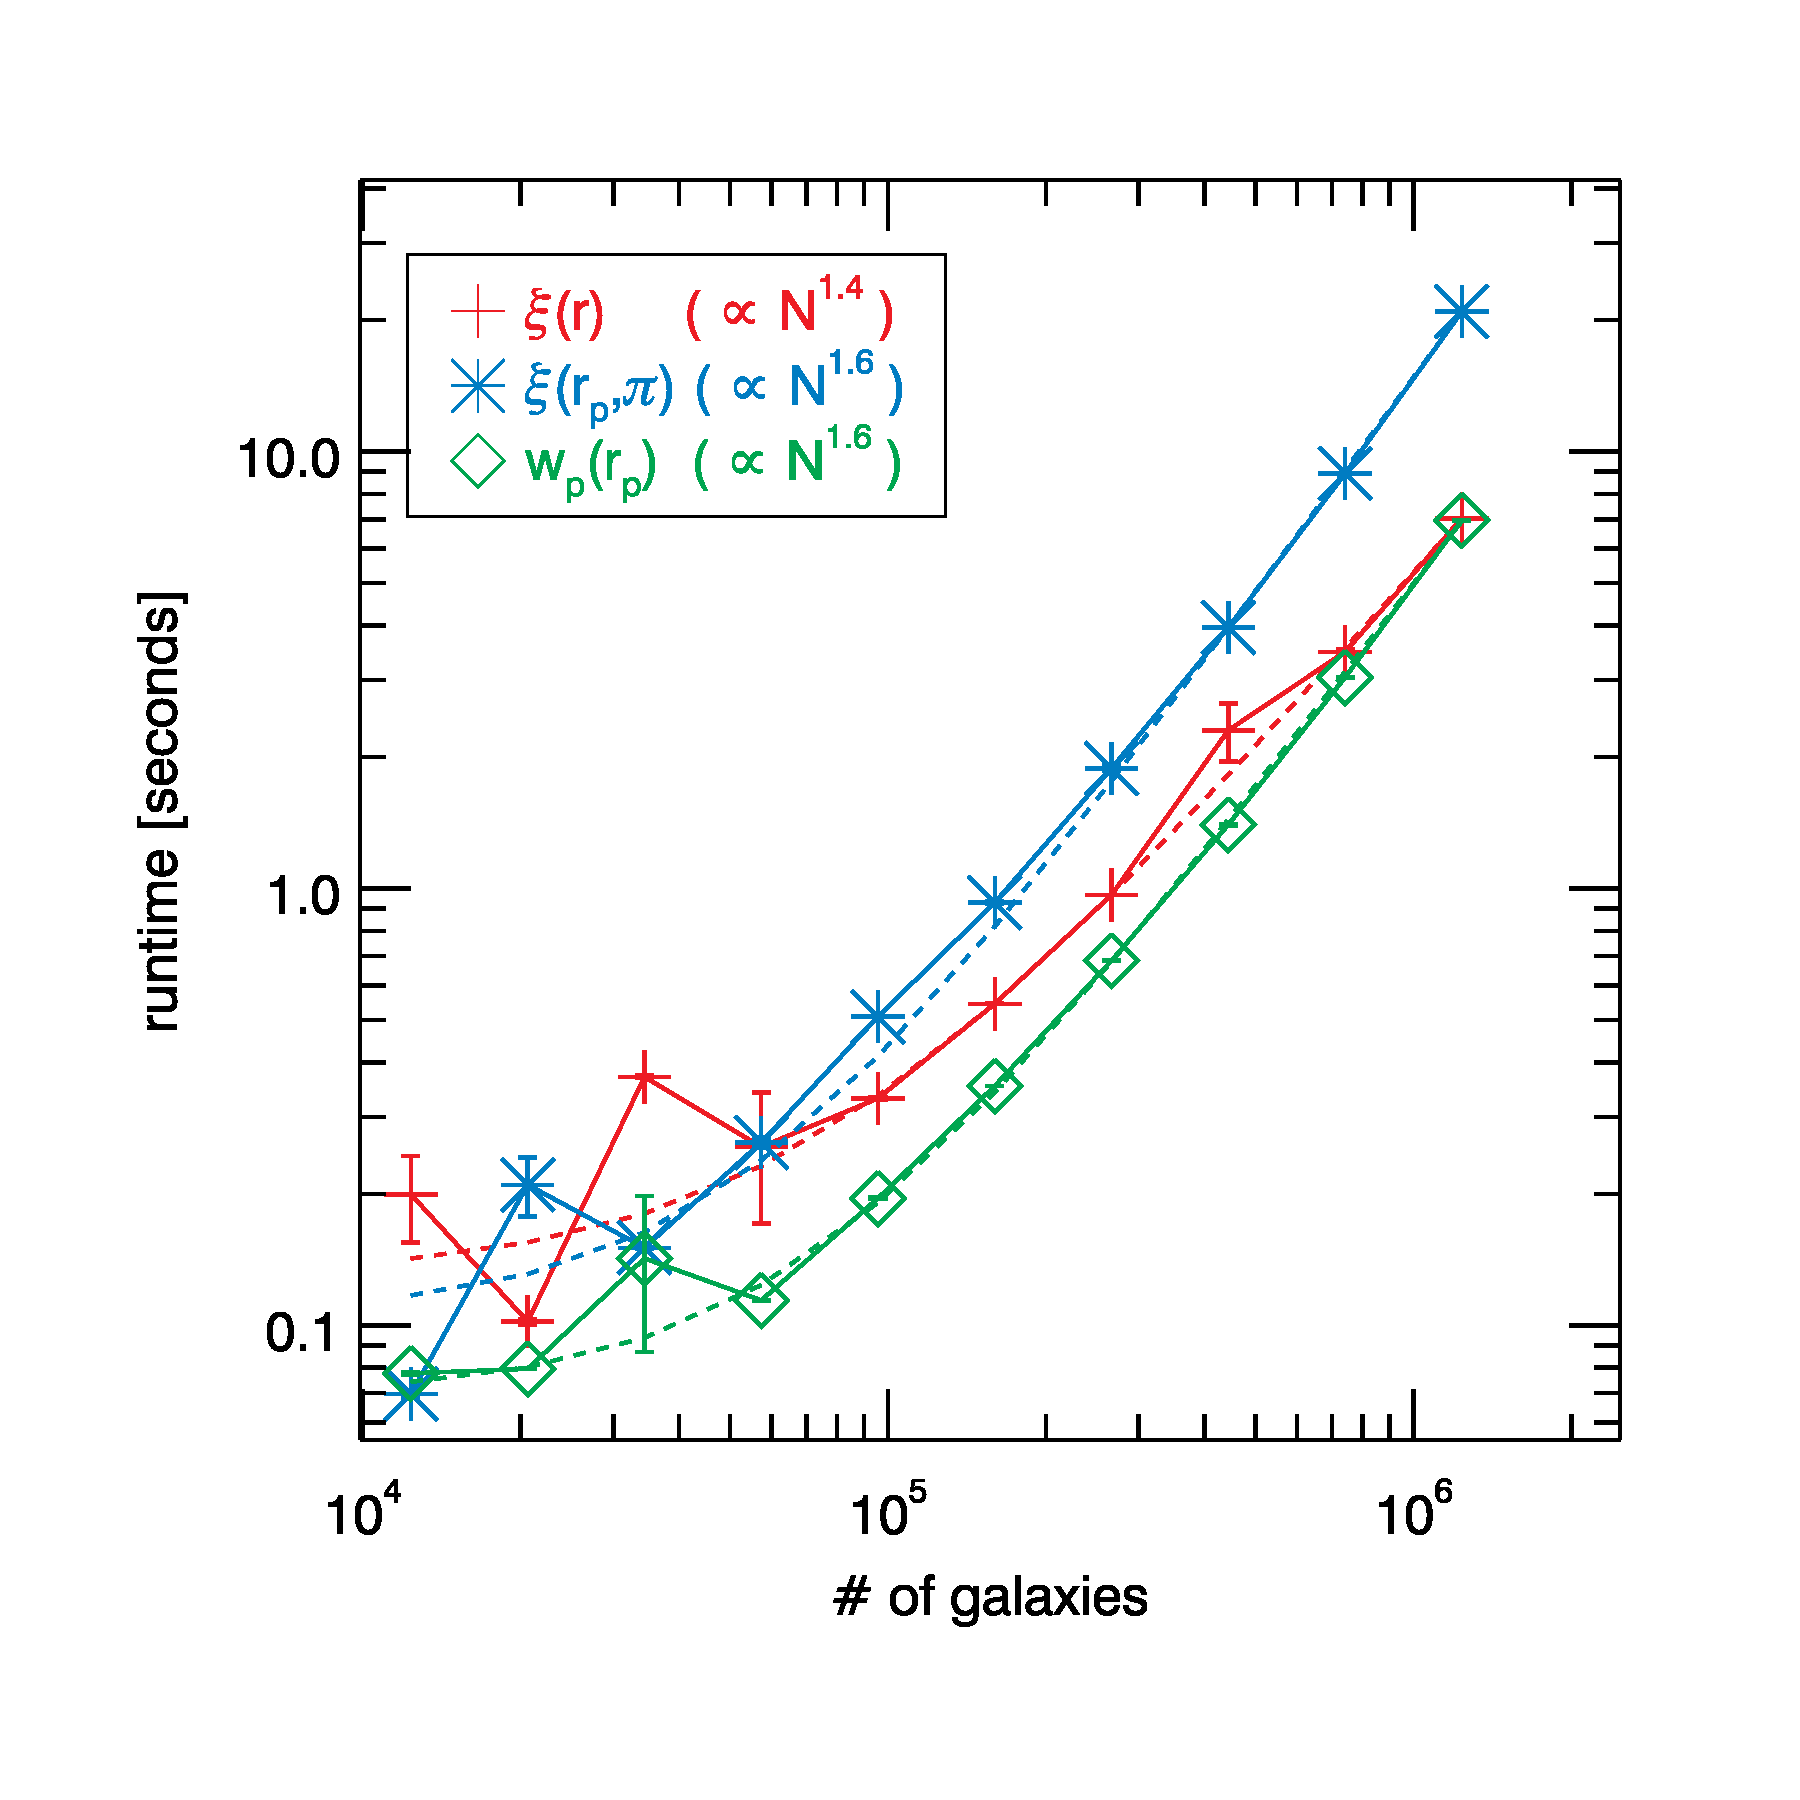
\includegraphics[clip=true,width=\linewidth]{timings_Mr19_numpart}%
\caption{Scaling with particle number for \xir, \xirppi, \wprp. The timings are obtained 
using 1 OpenMP thread. }
\label{fig:scaling_numpart}
\end{figure}

\subsection{Scaling with \texorpdfstring{\rmax}{rmax}}
The code runtime increases drastically as the largest requested separation, \rmax increases. Roughly speaking, the runtimes scale 
as $\mathcal{O}(r_{max}^2)$ with \xir showing the strongest dependence on \rmax. This is from the \pimax dependence of \xirppi and 
\wprp. Even when \rmax is large, the effective number of particles per cell only grows as $r_{max}^2$ and not $r_{max}^3$ (as it does 
for \xir). If we extend the benchmarks to larger \rmax, we will see a $\mathcal{O}(r_{max}^3)$ dependence for 
\begin{figure}[htbp]
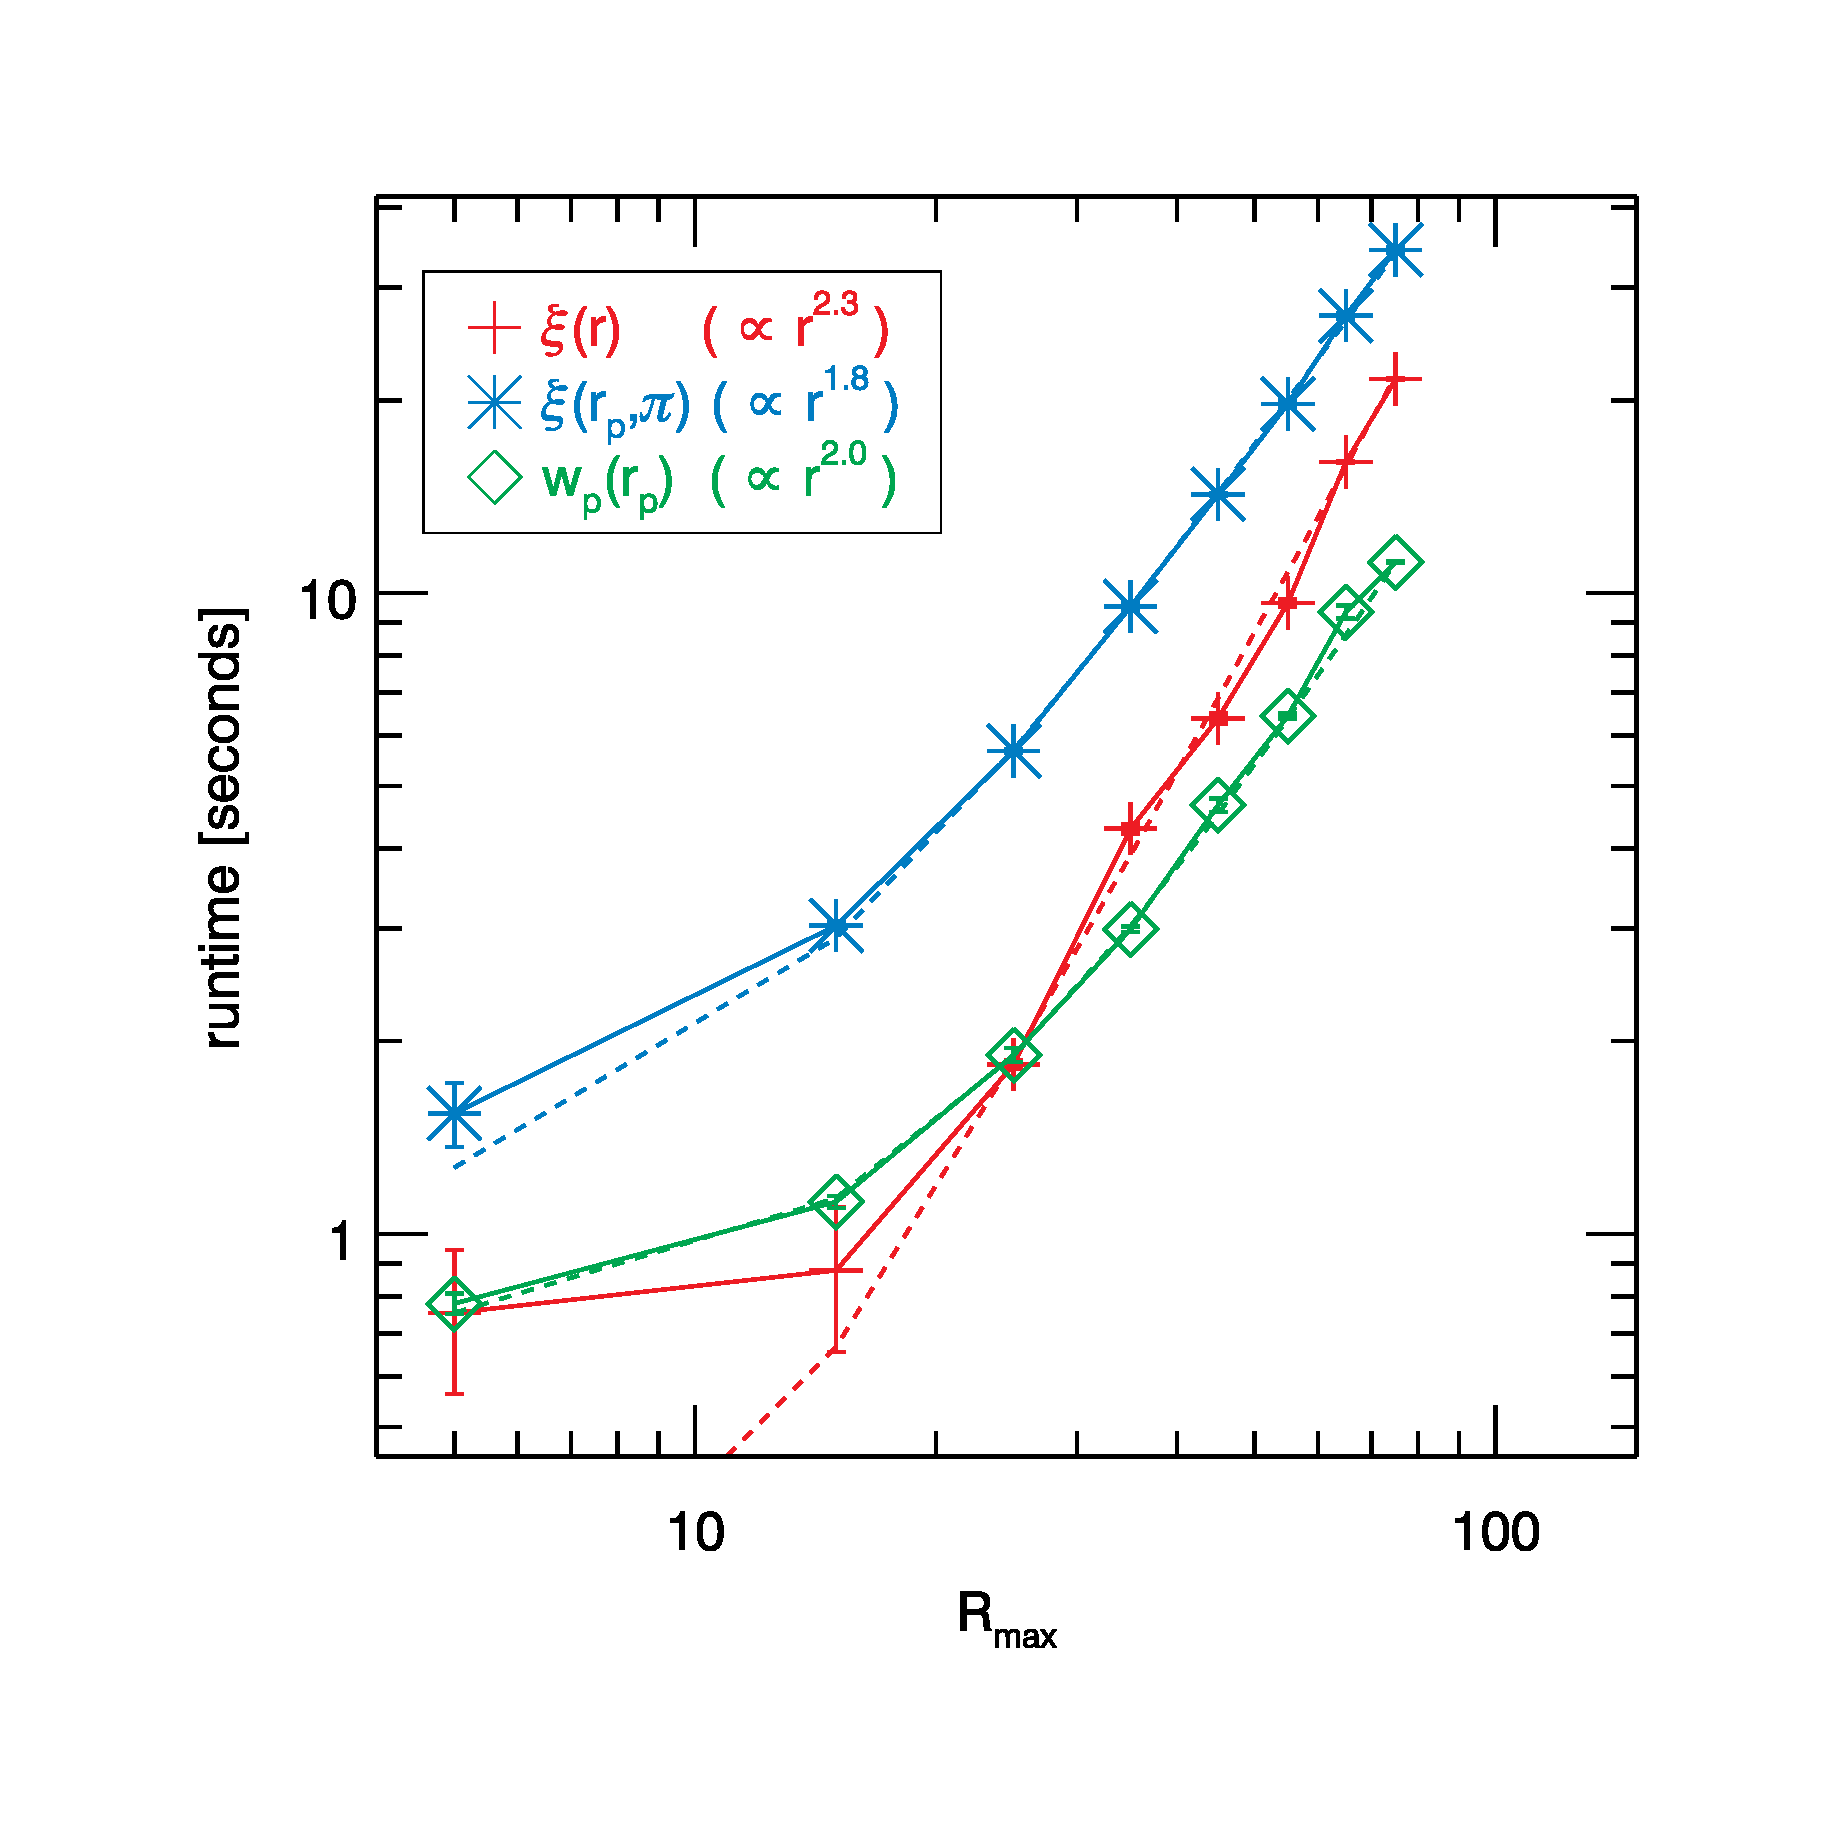
\includegraphics[clip=true,width=\linewidth]{timings_Mr19_rmax}%
\caption{Scaling with \rmax for \xir, \xirppi, \wprp. The timings are obtained 
with 4 OpenMP threads. }
\label{fig:scaling_rmax}
\end{figure}


\subsection{Scaling with OpenMP threads}
All of the codes presented here scale reasonably well (efficiency $\gtrsim$ 80\%) up to 10 OpenMP threads. Beyond that, the work-load is 
scaling efficiency starts dropping off and plateaus for \texttt{nthreads} $\gtrsim 20$. 
\begin{figure}[htbp]
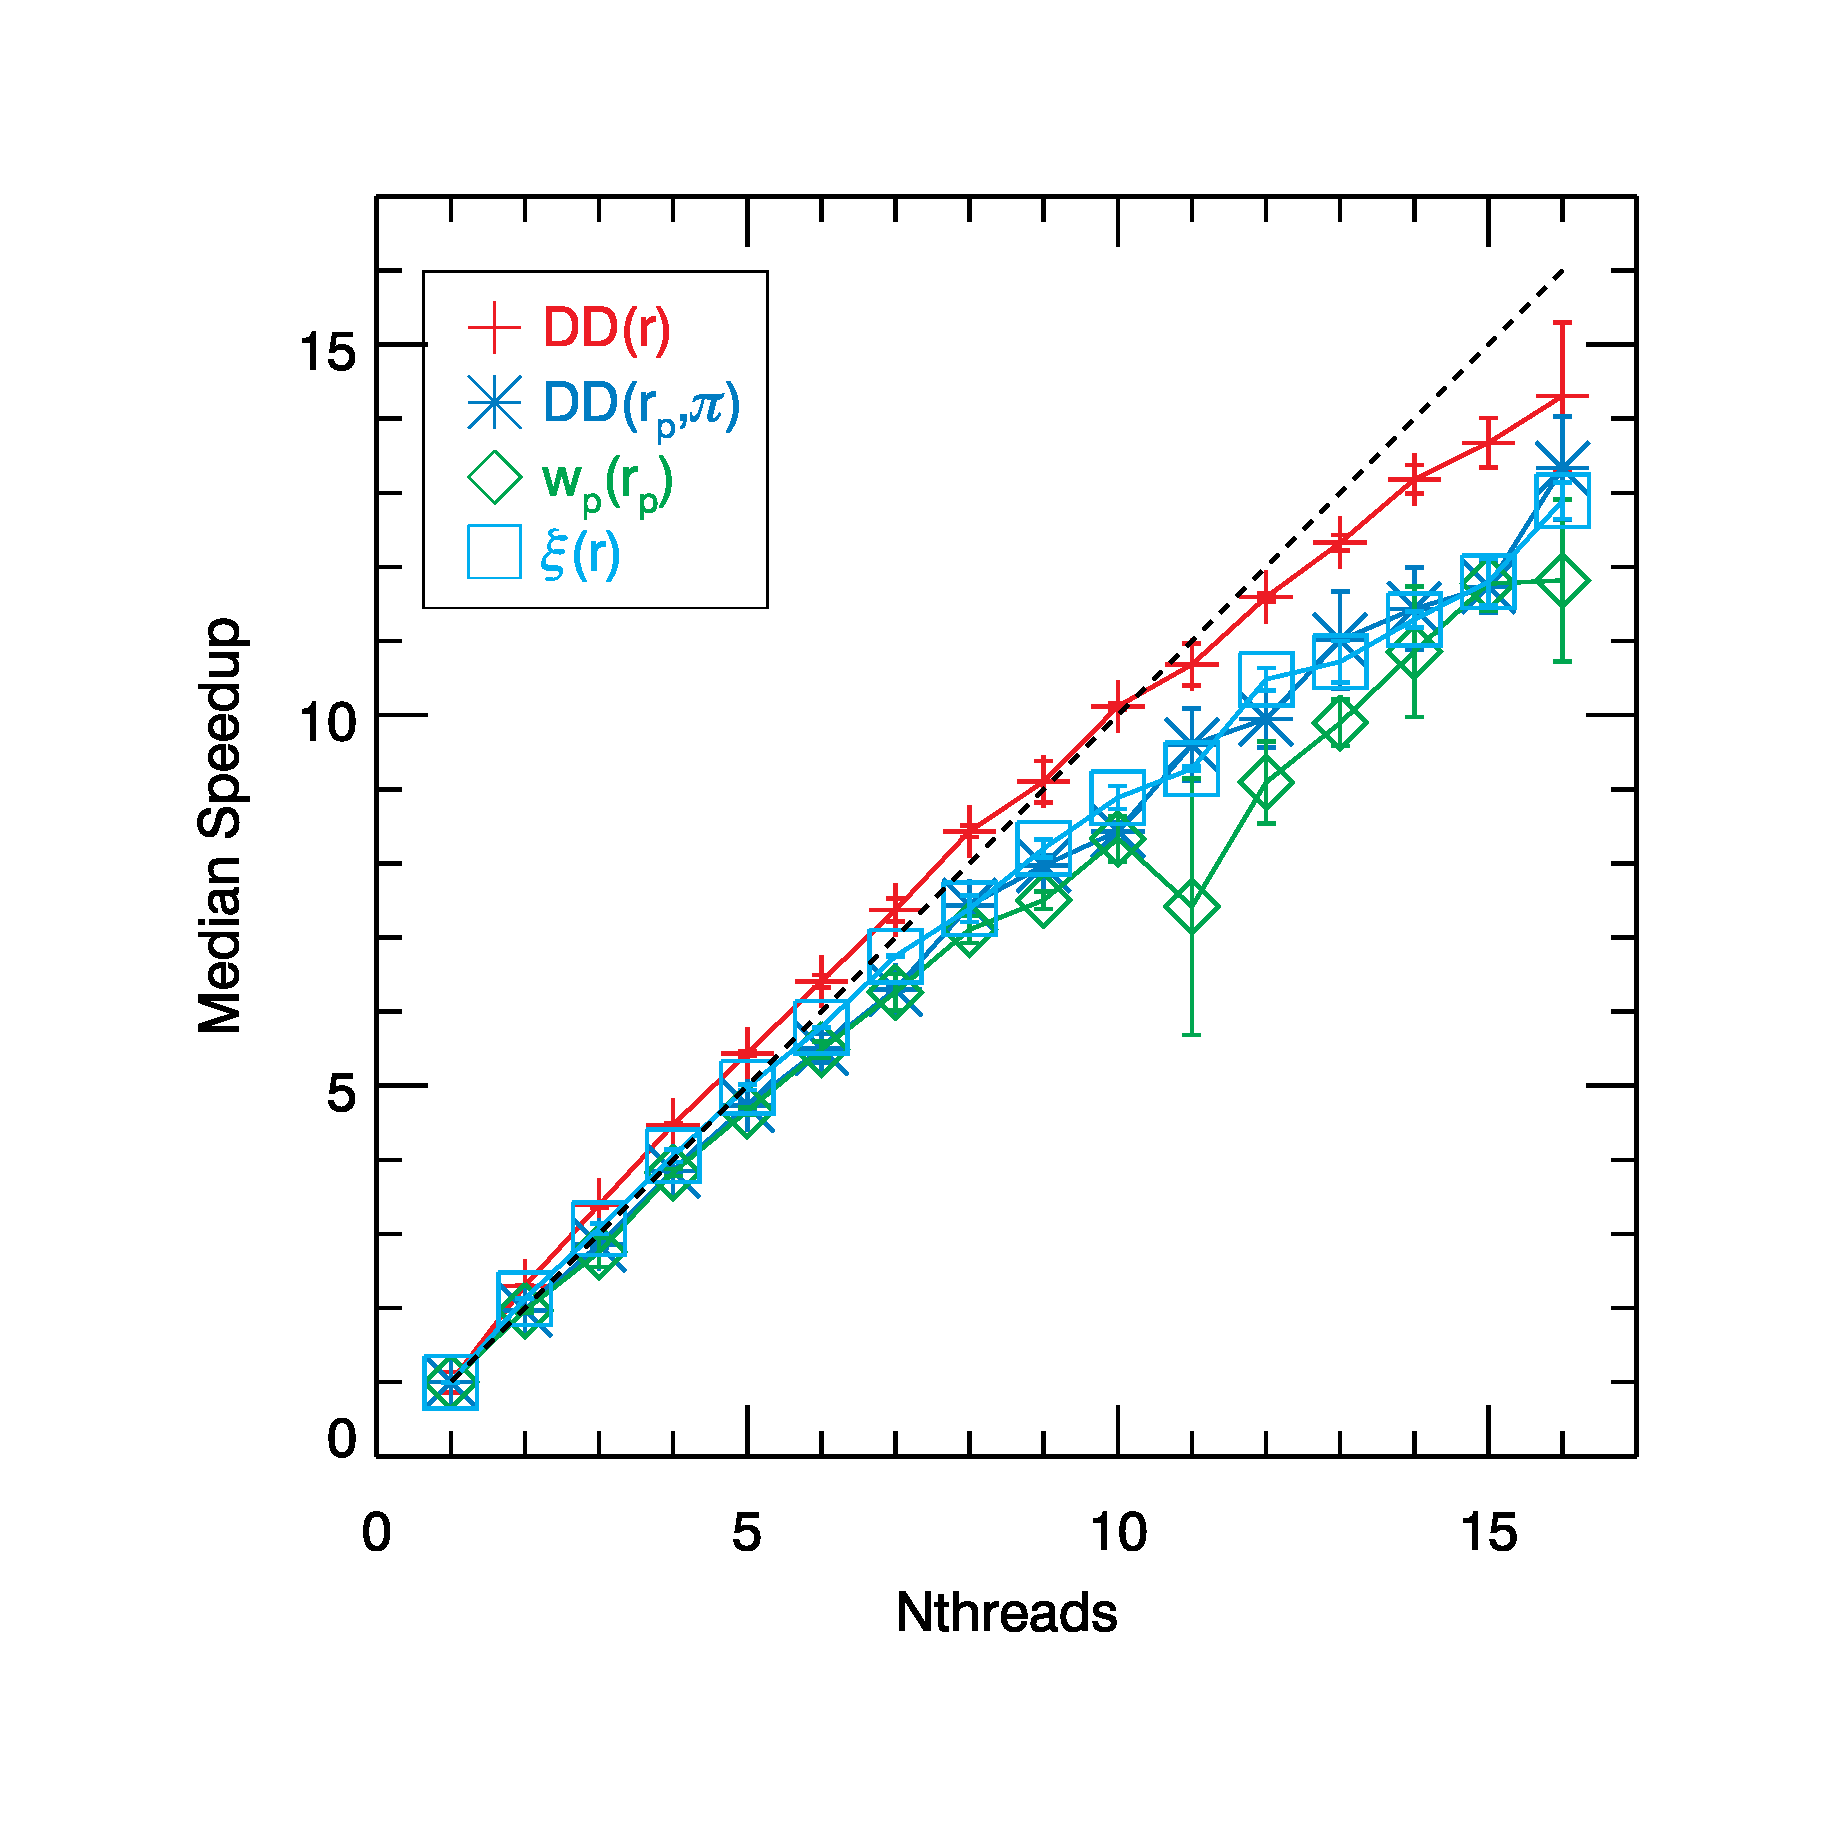
\includegraphics[clip=true,width=\linewidth]{timings_Mr19_openmp}%
\caption{OpenMP scaling for \xir, \xirppi, \wprp. The fiducial mock used here contains $\sim 10^6$ particles 
in a $420.0$ \hMpc cube. }
\label{fig:scaling_openmp}
\end{figure}

\begin{table}
\centering
\caption{\footnotesize OpenMP scaling for the three codes. Efficiencies are defined 
as \texttt{Speedup/Nthreads}. Note, that \xir has super-linear scaling with \texttt{nthreads}
up to $\sim$ 10 threads.}
\begin{adjustbox}{max width=\textwidth}
\begin{tabular}{ccccccccc} 
\toprule
\multirow{3}{*}{\textbf{Nthreads}}   &
\multicolumn{8}{c}{\textbf{Efficiency[\%]}} \\
\cmidrule(l{3em}r{3em}){2-9}

                                     &
\multicolumn{4}{c}{\textbf{Periodic Boxes}}  &
\multicolumn{4}{c}{\textbf{Spherical Geometry}}  \\
\cmidrule(l{1.0em}r{1.0em}){2-5}
\cmidrule(l{1.0em}r{1.0em}){6-9}
                                               &
\multicolumn{1}{c}{$\boldsymbol{\xir}$}        &
\multicolumn{1}{c}{$\boldsymbol{\xirppi}$}     &
\multicolumn{1}{c}{$\boldsymbol{\wprp}$}       & 
\multicolumn{1}{c}{$\boldsymbol{\xiofr}$}      &
\multicolumn{1}{c}{$\boldsymbol{DD(r_p,\pi)}$} &
\multicolumn{1}{c}{$\boldsymbol{DD(\theta)}$}  &
\multicolumn{1}{c}{$\boldsymbol{DR(r_p,\pi)}$} & 
\multicolumn{1}{c}{$\boldsymbol{DR(\theta)}$}   \\
\midrule
         1  &          100  &          100  &          100  &          100 &          100  &          100  &          100  &          100 \\
         2  &          115  &           98  &           98  &          106 &           96  &           94  &           97  &           98 \\
         3  &          113  &           95  &           91  &          102 &           91  &           83  &           91  &           92 \\
         4  &          111  &           96  &           95  &          101 &           85  &           78  &           92  &           89 \\
         5  &          108  &           94  &           93  &           99 &           87  &           76  &           86  &           87 \\
         6  &          106  &           91  &           91  &           96 &           89  &           70  &           84  &           77 \\
         7  &          105  &           90  &           89  &           96 &           84  &           68  &           97  &           80 \\
         8  &          105  &           92  &           88  &           92 &           76  &           59  &           95  &           75 \\
         9  &          101  &           88  &           83  &           91 &           72  &           65  &           89  &           75 \\
        10  &          101  &           84  &           83  &           88 &           72  &           57  &           78  &           75 \\
        11  &           97  &           87  &           67  &           84 &           74  &           56  &           77  &           69 \\
        12  &           96  &           82  &           75  &           87 &           70  &           53  &           79  &           69 \\
        13  &           94  &           84  &           76  &           82 &           67  &           47  &           73  &           71 \\
        14  &           94  &           81  &           77  &           80 &           67  &           44  &           78  &           63 \\
        15  &           91  &           78  &           78  &           78 &           62  &           43  &           66  &           61 \\
        16  &           89  &           83  &           73  &           80 &           57  &           44  &           66  &           58 \\

\bottomrule
\end{tabular}
\end{adjustbox}
\label{table:openmp}
\end{table}


\clearpage
\stdsection{Extending the Code}
\subsection{Different Type of Input Data File}
All of the codes use \texttt{io.c} in the \texttt{io} sub-directory to read-in the data. If you want to specify a different file format, the easiest way would be to edit 
\texttt{io.c}. Decide on the file format code and add another \texttt{strncmp} case in \texttt{io.c}. Remember that the \texttt{x/y/z} are declared as \texttt{void} pointers, 
so you can not directly reference the \texttt{x/y/z} pointers. If you do add support for a different file-type, please submit a pull request and I will be happy to merge it into the 
code-base. 

\subsection{Computing a different type of correlation function}
Let's say, you want to compute a marked correlation function. Now, you will need to read-in/create the marks for each individual point. Here are the steps 
you will need to create your custom correlation function code:
\begin{enumerate}
\item Add the data fields into the cellarray structure definition (see Listing~\ref{code:celldefn}.
\item Add in the memory allocation for the fields in \texttt{gridlink.c} after the \texttt{malloc} for \texttt{X/Y/Z} pointers (see Listing~\ref{code:malloc_cellarray}).
\item Extend \texttt{gridlink.c} to accept additional arrays and assign those arrays into \texttt{struct lattice} (see Listing~\ref{code:assign_to_cellarray}).
\item Enable OUTPUT\_RPAVG and DOUBLE\_PREC (this is not required, but probably the easiest way to create a custom correlation function calculation).
\item Declare and zero-initialize a \texttt{results} array that will contain your custom correlation function. Follow the implementation in the code for calculating \texttt{rpavg}.
\item Add in the AVX arrays that load your custom data fields in the \texttt{j loop} in the \texttt{countpairs*} functions.
\item Add your custom correlation function weight into the \texttt{results} array. Combine thread-local arrays into a global one in case USE\_OMP is selected. 
\item Add the custom correlation function field to the corresponding \texttt{struct results\_countpairs*}. Assign the \texttt{results} array into the \texttt{struct results\_countpairs*}.
\item Add a call to \texttt{free(your field)} in the corresponding function \texttt{free\_results\_countpairs*}.
\end{enumerate}

\subsection{Using SSE instead of AVX}
If your CPU is too old and does not support AVX, then you can still use SSE instrinsics to compute the correlation functions. However, this will require replacing all of the 
AVX sections with corresponding SSE intrinsics. \href{mailto:manodeep@gmail.com}{Email me} and I will guide you through the conversion process. 

%% \bibliographystyle{apj}
%% \bibliography{master}

\section{License}
The code has been released under the MIT License. 
\begin{verbatim}
Permission is hereby granted, free of charge, to any person 
obtaining a copy of this software and associated documentation 
files (the ``Software''), to deal in the Software without 
restriction, including without limitation the rights to use, 
copy, modify, merge, publish, distribute, sublicense, and/or
sell copies of the Software, and to permit persons to whom 
the Software is furnished to do so, subject to the following 
conditions:

The above copyright notice and this permission notice shall 
be included in all copies or substantial portions of the 
Software.

THE SOFTWARE IS PROVIDED ``AS IS'', WITHOUT WARRANTY OF ANY 
KIND, EXPRESS OR IMPLIED, INCLUDING BUT NOT LIMITED TO THE 
WARRANTIES OF MERCHANTABILITY, FITNESS FOR A PARTICULAR 
PURPOSE AND NONINFRINGEMENT. IN NO EVENT SHALL THE AUTHORS 
OR COPYRIGHT HOLDERS BE LIABLE FOR ANY CLAIM, DAMAGES OR 
OTHER LIABILITY, WHETHER IN AN ACTION OF CONTRACT, TORT 
OR OTHERWISE, ARISING FROM, OUT OF OR IN CONNECTION 
WITH THE SOFTWARE OR THE USE OR OTHER DEALINGS IN 
THE SOFTWARE.
\end{verbatim}

\end{document}




